\chapter{Beszédadatbázisok}

A fejezet bemutatja a jelenleg ingyenes, bárki által elérhető és a tanítás során használt beszédadatbázisokat. Egy beszédadatbázis előállítása bár ránézésre egyszerű feladatnak tűnik,
valójában komplex folyamat és sok munkát igényel. Egyes adatbázisokat beszédfelismerés céljából készítettek, másokat beszélőfelismerésre. Az előbbinél a kontrollált körülmények előállítása, megfelelés egyes nyelvtani mérőszámoknak (fonémák, diádok egyenletes elosztása stb.), utóbbinál a nagyobb méret miatt az automatizmus szükségessége bonyolítja a feladatot. Ezen felül mindkét esetben a szerzői jogok védelmére is ügyelni kell. (A dolgozatban a beszédadatbázis, beszédkorpusz és beszédadathalmaz ugyanarra vonatkozik.)

\section{Beszédadatbázisok}

\subsection{TIMIT}

A TIMIT beszédkorpuszt automatikus beszédfelismerő rendszerek fejlesztéséhez tervezték. 630 beszélőtől tartalmaz mintákat amerikai angol nyelven a 8 legelterjedtebb nyelvjárásban.
A TIMIT archívum tartalmaz egy TRAIN és egy TEST mappát, ezek tanításhoz és teszteléshez valók. Ezeken belül további, a dialektusok sorszámával (DR1, ..., DR8), azon belül a beszélő azonosítójával elnevezett könyvtárak találhatók. Egy beszélőhöz
10 db beszédminta tartozik 16 kHz-es NIST SPHERE fájlok formájában~\cite{timit}.
\newline
\newline
\begin{table}[!ht]
	\begin{tabular}{*4l} \toprule
		\bfseries Dialektus regió (DR) & \bfseries Férfi & \bfseries Nő & \bfseries Összesen \\ \midrule
		1                             & 31 (63\%)      & 18 (27\%)   & 49 (8\%)          \\
		\rowcolor{gray!10} 
		2                             & 71 (70\%)      & 31 (30\%)   & 102 (16\%)        \\
		3                             & 79 (67\%)      & 23 (23\%)   & 102 (16\%)        \\
		\rowcolor{gray!10} 
		4                             & 69 (69\%)      & 31 (31\%)   & 100 (16\%)        \\
		5                             & 62 (63\%)      & 36 (37\%)   & 98 (16\%)         \\
		\rowcolor{gray!10} 
		6                             & 30 (65\%)      & 16 (35\%)   & 46 (7\%)          \\
		7                             & 74 (74\%)      & 26 (26\%)   & 100 (16\%)        \\
		\rowcolor{gray!10} 
		8                             & 22 (67\%)      & 11 (33\%)   & 33 (5\%)          \\
		\bottomrule
		\hline
	\end{tabular}
	\centering
	\caption{A beszélők eloszlása dialektusok szerint.}
	\label{fig:timit-dialects}
\end{table}
\newpage
A dialektus régiók a következők:

\begin{multicols}{2}
	\begin{itemize}
		\item DR1:  New England
		\item DR2:  Northern
		\item DR3:  North Midland
		\item DR4:  South Midland
		\item DR5:  Southern
		\item DR6:  New York City
		\item DR7:  Western
		\item DR8:  Army Brat (moved around)
	\end{itemize}
\end{multicols}
\ \\
A NIST SPHERE formátum az elején definiál egy fix hosszú fejlécet, amit a hang bináris kódolása követ. Erre figyelni kell a hangfájlok beolvasásánál, Python esetében nem minden hangfeldolgozó könyvtár támogatja. Ilyen esetben kézzel el kell távolítani a fejlécet a fájlok elejéről. A hangfájlokhoz tartozik egy szöveges dokumentum ami az elhangzott szöveget és annak a wav fájlbeli helyét tartalmazza. Továbbá egy WRD fájl írja le a szavakat és egy PHN kiterjesztésű a fonémákat, illetve azok időbeni elhelyezkedését a wav fájlban.
\newline
\newline
A hangfájlokhoz tartozó egyéb fájlok beszédfelismerés szempontjából fontosak. Mivel én a beszédkorpuszt beszélőfelismerésre használtam, csak a hangfájlokra volt szükségem. A TEST mappában -- mivel a TIMIT-et alapvetően beszédfelismeréshez tervezték -- teljesen különböző beszélők vannak a TRAIN mappához képest, ezért a TRAIN mappabeli beszélőket osztottam fel tanításhoz és teszteléshez.

\subsection{CMU Arctic}

A CMU Arctic adatbázist beszédszintézishez kapcsolódó kutatásokhoz tervezték. A beszédszintézis az emberi beszéd mesterséges, általában számítógéppel történő előállítása. Mivel akkoriban (2003) a publikusan elérhető beszédadatbázisok kis méretűek voltak, létrehozták a CMU Arcticot, ami több beszédadatbázis összessége. Egy adatbázis egy beszélőhöz tartozik és egyéb információkat is tartalmaz, mint a fonetikus kiejtés vagy a beszédjel egyes jellemzőit (pitchmark) tartalmazó fájlok~\cite{cmu_arctic}.
\newline
\newline
Mivel a CMU Arctic felhasználási célja a beszédszintézis, a felvételek studió minőségűek, mentesek külső zajoktól és a beszélő által keltett zajoktól is.
\newline
\newline
Az egyes Arctic adatbázisok közel 1150 kb. 1-4 másodperces beszédmintából állnak. Az egy beszélőhöz tartozó mintákat két azonos elemszámú A és B csoportra osztották, amelyek fonetikailag kiegyensúlyozottak. Ez azt jelenti, hogy az adott beszédmintában található fonémák körülbelül ugyanakkora gyakorisággal fordulnak elő mint az átlagos társalgás közben az adott nyelven.
A beszédminták WAV fájlok formájában 32 kHz-en lettek mintavételezve. A felvételek öt beszélőtől tartalmaznak hangmintákat:
\newline
\begin{itemize}
	\item férfi általános amerikai angol akcentus
	\item női általános amerikai angol akcentus
	\item férfi kanadai angol akcentus
	\item férfi skót angol akcentus
	\item férfi indiai angol akcentus
\end{itemize}
\bigskip
A CMU Arctic tartalmaz egy listát az egyes beszélők által felolvasott szövegekkel.
Mivel ez egy mindenki által elérhető ingyenes beszédadatbázisnak készült és szabad szoftver licensszel rendelkezik, fontos szempont volt, hogy a felolvasott szövegek ne sértsenek szerzői jogokat. Emiatt a listán szereplő mondatok a legnagyobb ingyenes, szabadon felhasználható szövegkorpuszból, a Project Gutenbergből származnak. A Project Gutenberg célja szerzői jogokat nem sértő angol nyelvű könyvek gyűjtése és elérhetővé tétele.
\newline
\newline
A CMU Arctic eleinte 2,5 millió szóból és az azokat tartalmazó 168000 mondatból állt. Ezekből a FestVox beszédszintézis projekt segítségével kiválogattak 52000 olyan mondatot, amelyek kiejtése könnyű és hossza 5 és 15 szó közé esett. További szigorításként csak olyan szavak kerülhettek be, amelyek részei a CMUDICT lexikonnak, hogy elkerüljék az eltérő kiejtéseket.
\newline
\newline
Ezután a Festvox segítségével az 52000 mondatból kiválogatták a legnagyobb diád lefedettségű halmazt. A diád két egymás utáni félhang együtteseként előálló nyelvi egység, amely lefedettségének mértéke a beszédszintézis során előállított beszéd minősége miatt fontos. 
\newline
\newline
A kiválogatott részt kivéve egy újabb halmazt választottak ki, amelyek 668 és 629 mondatból álltak. Ezeket manuálisan átnézve tovább finomították.

\begin{table}[!ht]
	\begin{tabular}{*4l} \toprule
		\bfseries Arctic & \bfseries Automatikus fázis & \bfseries Kézi finomítás I. & \bfseries Kézi finomítás II. \\ \midrule
		A halmaz                             & 668      & 597   & 593          \\
		\rowcolor{gray!10} 
		B halmaz                             & 629      & 541   & 539        \\
		Összesen                             & 1297      & 1138   & 1132        \\
		\bottomrule
		\hline
	\end{tabular}
	\centering
	\caption{Arctic CMU automatikus és kézi fázisok.}
	\label{fig:arctic-phases}
\end{table}
\ \\
A CMU Arctic diád lefedettsége 80\% és az előbbihez hasonlóan triád lefedettsége 14\%. Az előbbi megelőzi a TIMIT beszédkorpuszban lévő diád lefedettséget, utóbbiban viszont a TIMIT jobb a több (2343) mondat miatt.

\begin{table}[!ht]
	\begin{tabular}{*8l} \toprule
		\bfseries Corpus & \bfseries Mondat & \bfseries Szó & \bfseries Fonéma  & \bfseries \begin{tabular}{@{}l@{}} Fonéma \\ lefedettség \end{tabular}  & \bfseries \begin{tabular}{@{}l@{}} Diád \\ lefedettség \end{tabular}  & \bfseries \begin{tabular}{@{}l@{}} Triád \\ lefedettség \end{tabular} \\ \midrule
		TIMIT-all & 2342 & 20771 & 87819 & 100\% & 78,2\% & 19,4\% \\
		\rowcolor{gray!10} 
		Arctic & 1132 & 10045 & 39153 & 100\% & 79,6\% & 13,7\% \\
		\bottomrule
		\hline
	\end{tabular}
	\centering
	\caption{Arctic CMU vs. TIMIT.}
	\label{fig:arctic-vs-timit}
\end{table}

\subsection{LibriSpeech}

2015-ben már vizsgálták a hangoskönyvek beszédszintézishez való használatát és léteztek ilyen célú beszédadatbázisok, de nem volt automatikus beszédfelismerés céljára létrehozott, ingyenes, mindenki által elérhető beszédkorpusz. A LibriSpeech beszédfelismerő rendszerek tanítására és kiértékelésére készült. Tartalma a LibriVox projektből származik, amelynek célja szabadon terjeszthető hangfelvételek készítése ingyenes, közkinccsé vált könyvekről, és ezek közzététele bárki számára az interneten~\cite{librispeech}.
\newline
\newline
A projekt körülbelül 1000 órányi beszédet tartalmaz 16 kHz-en mintavételezve. Tartalmaz ezek mellett több előre tanított beszédfelismerő modellt és Kaldi szkripteket beszédfelismerő rendszerek készítéséhez.
\newline
\newline
Az előfeldolgozási fázisban a könyvek szövegét normalizálták; kis és nagybetűk helyett csak nagybetűket használtak, eltüntették az írásjeleket és a gyakori rövidítéseket teljes szavakkal helyettesítették. Ezután a hangmintákat felismertették a Kaldi \emph{gmm-decode-faster} dekóderével, amihez egy VoxCeleb adatbázison tanított modellt használtak.
\newline
\newline
Összemérték az előbbi modell által felismert szöveget az eredeti írással és azokat a részeket választották ki, ahol a kettő megegyezett. A hanganyagot legfeljebb 35 másodperces részekre tördelték minimum 0.5 másodperces szünetek mentén.
\newline
\newline
A következő fázisban egy fMMRl (HMM-alapú) modellel ismét összemérték a felismert szöveget a valódival. Ez okozott hamis pozitív eredményeket is, de az audioanyag mennyisége miatt elhanyagolható volt. Ez a fázis tehát 35 másodperces nagy valószínűséggel helyesen transzkriptált anyagokat tartalmazott.
\newline
\newline
A harmadik fázis ezeknek az apróbb szegmensekre tördelése volt, amit két módszerrel végeztek el. Tanítóadatok esetén minden olyan szünetnél tördeltek, ahol az legalább 0,3 másodperc hosszú volt. Tesztadatok esetén csak ott tördeltek, ahol ez a szünet egybeesett a mondat végével is.

\begin{table}[!ht]
	\begin{tabular}{*6l} \toprule
		\bfseries Részhalmaz & \bfseries Óra & \bfseries beszélő / perc & \bfseries \begin{tabular}{@{}l@{}} Férfi \\ beszélő \end{tabular}
		& \bfseries \begin{tabular}{@{}l@{}} Női \\ beszélő \end{tabular} & \bfseries \begin{tabular}{@{}l@{}} Összes \\ beszélő \end{tabular} \\ \midrule
		dev-clean & 5,4 & 8 & 20 & 20 & 40 \\
		\rowcolor{gray!10} 
		test-clean & 5,4 & 8 & 20 & 20 & 40 \\
		dev-other & 5,3 & 10 & 16 & 17 & 33 \\
		\rowcolor{gray!10} 
		test-other & 5,1 & 10 & 17 & 16 & 33 \\
		train-clean-100 & 100,6 & 25 & 125 & 126 & 251 \\
		\rowcolor{gray!10}
		train-clean-360 & 363,6 & 25 & 439 & 482 & 921 \\
		train-other-500 & 496,7 & 30 & 564 & 602 & 1166 \\
		\bottomrule
		\hline
	\end{tabular}
	\centering
	\caption{LibriSpeech részhalmazok.}
	\label{fig:librispeech-subset}
\end{table}
\ \\
Az audiófelvételek válogatásához a LibriVox API segítségével szereztek információkat a felolvasóról,
hogy mely hangoskönyvekben olvastak fel milyen fejezeteket, a kapcsolódó referencia szövegeket pedig a Project  Gutenbergből és az Internet Archiveból nyerték ki. A \emph{train}, \emph{dev} és \emph{test} részhalmazok között fontos, hogy ne legyen átfedés, tehát ugyanaz az olvasó csak egyetlen halmazban olvasson ezek közül. Ehhez a válogatáson kívül további óvintézkedésként kivették a többszereplős fejezeteket és lefuttaták a LIUM beszélő szegmentáló toolkitet ennek detektálására.
\newline
\newline
A tanítóhalmazba válogatott részeket három részre osztották. Ezek egyenként 100, 360 és 500 órányi audiofelvételt tartalmaznak. Az első kettőbe automatikus módszerrel az amerikai angol akcentushoz hasonló részeket válogatták bele. Egy egyszerű, a Wall Street Journal si-84 adatbázison tanított akusztikus modellt használtak a LibriSpeechen beszédfelismerésre. Ezáltal meghatározták és rangsorolták a beszélőket a Word Error Rate (a modell által hibásan felismert szavak) szerint. Az alacsonyabb WER pontszámmal rendelkező olvasók a \emph{clean}, a magasabbal az \emph{other} részhalmazokba kerültek.

\subsection{VoxCeleb1} \label{voxceleb1}

A beszélőfelismerésre használt adatbázisok kontrollált körülmények között felvett audio anyagot tartalmaznak és kézzel válogatottak, emiatt kis méretűek. Kontrollált körülmény alatt értjük a studioban felvett, külső és belső zajoktól mentes hanganyagot. Ezek a valós körülmények közötti, azaz zajos környezetben elhangzó beszédfelismerést megnehezítik. A VoxCeleb készítői a beszélőfelismerő adabázisok automatikus létrehozására terveztek egy folyamatot és létrehozták, valamint ingyenesen elérhetővé tették a VoxCeleb beszédadatbázist, ami valós körülmények közötti hangfelvételeket tartalmaz~\cite{voxceleb1}.
\newline
\newline

\begin{table}[!ht]
	\begin{tabular}{*4l} \toprule
		\bfseries Név & \bfseries Körülmények & \bfseries Beszélők száma & \bfseries Minták száma \\ \midrule
		ELSDSR                             & Kontrollált & 22     & 198          \\
		\rowcolor{gray!10} 
		Forensic Comparison                & Telefonos   & 552   & 1264        \\
		SITW                           & Multimédia        & 299   & 2800        \\
		\rowcolor{gray!10} 
		VoxCeleb                           & Multimédia        & 1251   & 153516        \\
		\bottomrule
		\hline
	\end{tabular}
	\centering
	\caption{Beszédadatbázisok beszédfelismerés.}
	\label{fig:speaker-recognition-datasets}
\end{table}
\ \\
A VoxCeleb több mint 100000 olyan beszédmintát tartalmaz 1251 hírességtől, amik YouTube videókból származnak. Az adatbázisban a nemek aránya kiegyensúlyozott (férfiak 55\%, nők 45\%), a beszélők különböző származásúak, korúak illetve eltérő akcentussal rendelkeznek. A beszéd általában publikus eseményekről származik, így a háttérzaj, egyéb beszélők és a felvevő eszköz minősége zajossá teszi azt.
\newline
\newline
Az adatbázis előállítása a következő módon történt:
\begin{itemize}
	\item A beszélő jelöltek kiválasztása:  Olyan hírességeket válogattak akik benne vannak a VGG adathalmazban, ami 2622 híres (interneten sokat keresett) ember arcát tartalmazza.
	\item YouTube videók letöltése: Letöltötték a kiválasztott emberekhez tartozó első 50 YouTube videót. A keresés az illető nevét és utána az \emph{interview} szót tartalmazta, hogy kiszűrjék a zeneszámokat, sportfelvételeket és minél nagyobb valószínűséggel beszéljenek benne.
	\item Arcdetektálás: Az egyes videókon egy HOG-alapú arc detektorral meghatározták az arcok helyét minden egyes frameben.
	\item Aktív beszélőazonosítás: Mivel egy videóban több arc is megjelenhet egyszerre, vagy a beszélőt szinkronizálhatják, az éppen beszélő arc meghatározására illetve a szinkron kiszűrésére volt szükség. A megoldás a SyncNet volt, egy olyan kétcsatornás CNN, ami képes megbecsülni a szájmozgás és a beszéd közötti korrelációt.
	\item Arcfelismerés: Végül egy a VGG Face adathalmazzal tanított CNN segítségével ellenőrizték, hogy a beszélő arc valóban a kérdéses személy-e.
\end{itemize}

\subsection{VoxCeleb2} \label{voxceleb2}

A VoxCeleb2 ugyanúgy beszélőfelismeréshez készített, de az előző verzióhoz képest jóval nagyobb, 6112 hírességtől tartalmaz 2442 órányi beszédet tartalmazó beszédadatbázis különböző nyelvű, korú és származású beszélőkkel~\cite{voxceleb2}.
\newline
\newline
Az adatbázis előállítási folyamatot az előzőhöz képest tovább bővítették.
\begin{itemize}
	\item Duplikátum detektálás: YouTube-on gyakran feltöltik ugyanazt a videót más url alatt különböző felhasználók. Egy a VoxCeleb1 adatbázison tanított konvolúciós hálózatot használtak jellemző kinyerésre, amellyel 1024 dimenziós vektorokkal reprezentálták a beszédmintákat. Egy beszélőre kiszámolták a vektorpárok közötti Euklideszi-távolságot és ahol ez kisebb volt mint 0,1 azokat azonosnak tekintették.
	\item Nemzetiség: A beszélők nemzetiségét a Wikipediáról gyűjtötték ki egy keresőrobottal (angolul webcrawler). Ezzel a módszerrel a 6112 beszélő közül 5689 nemzetiségét sikeresen azonosították. Ebből kiderült, hogy a VoxCeleb2 etnikailag sokkal diverzifikáltabb a VoxCeleb1-hez képest, mivel a VoxCeleb1 adatbázisban jelenlévő 36 nemzetiségnél jóval többet, pontosan 145-öt tartalmaz. Ugyanakkor az amerikai angolt beszélők aránya is sokkal kisebb, 29\% a VoxCeleb1-ben mért 64\%-hoz képest.
\end{itemize}

\begin{table}[!ht]
	\begin{tabular}{*3l} \toprule
		\bfseries Adatok & \bfseries VoxCeleb1 & \bfseries VoxCeleb2 \\ \midrule
		Beszélők száma   & 1251 & 6112 \\
		\rowcolor{gray!10} 
		Beszélők száma   & 1251 & 6112 \\
		Női beszélők száma & 561 & 2351 \\
		\rowcolor{gray!10}
		Férfi beszélők száma & 690 & 3761 \\
		Videók száma & 22496 & 150480 \\
		\rowcolor{gray!10}
		Beszédminták száma & 153516 & 1128246 \\
		Átlagos videó / beszélő & 18 & 25 \\
		\rowcolor{gray!10}
		Átlagos beszédminta / beszélő & 116 & 185 \\
		Átlagos beszédminta hossz & 8,2 & 7,8 \\
		\bottomrule
		\hline
	\end{tabular}
	\centering
	\caption{VoxCeleb1 vs. VoxCeleb2.}
	\label{fig:voxceleb1-vs-2}
\end{table}

\chapter{Neurális hálózat alapú beszélőfelismerő rendszerek}

Ebben a fejezetben bemutatom a legújabb korszerű, mély neurális hálózaton alapuló beszélőfelismerő rendszereket, majd ismertetem a WaveNet architektúrát és egy arra épülő beszélőfelismerő neurális hálózatot; a Wavenet classifiert. Végül bemutatom a voicemapet, egy beszélőfelismerő feladatokra használható könyvtárat, amelyet a saját alkalmazásomban is felhasználok. Az előbbi két rendszeren saját méréseket is végzek.
\newline
\newline
Fontos különbség, hogy míg a WaveNet classifier csupán zárthalmazú beszélőfelismerésre képes, a voicemap más elven, hangvektorokkal működik, ezért támogatja a nyílthalmazú beszélőfelismerést.

\section{Modern beszélőfelismerés} \label{section:modern_speaker_recognition}

A következő fejezetben bemutatom a 2017-2019-ben publikált korszerű beszélőfelismerő rendszereket és az általuk elért eredményeket. Mivel ez a kutatási terület jelenleg népszerű és folyamatosan újabb eredményeket érnek el, a bemutatott rendszereket a hivatkozások száma, a dátum és a \emph{www.paperswithcode.com} oldal rangsorolása alapján választottam ki.
\newline
\newline
Az eredmények általános összehasonlítása több ok miatt is nehéz feladat. A cikkekben a legjobb eredmények feltüntetése miatt relatív eredményeket tartalmaznak egy-egy korábban
publikált rendszerhez képest. Ezen kívül változik, hogy zárt vagy nyílt-halmazú beszélőfelismerésről, beszélő azonosításról vagy beszélő-ellenőrzésről van-e szó. Változik maga a teszthalmaz nehézsége is: etnikai, nemi, foglalkozásbeli diverzitás, a hangminták hossza, a hangfelvétel minősége, van-e irreleváns zaj, stb. Továbbá
a legtöbb cikk nem biztosít letölthető modellt, konfigurációt, szkripteket az előfeldolgozáshoz, így azonos környezethez reprodukálni kellene őket.


\subsection{Deep Speaker: an End-to-End Neural Speaker Embedding System}

A Deep Speaker (2017) egy neurális hálózatokon alapuló embedding rendszer. Az \emph{embedding} kifejezés alatt valamilyen leképzést értünk. Például amikor hangokból hangvektorokat készítünk. A rendszer a hangmintákat egy hipergömbre vetíti, ahol azoknak a hasonlóságát koszinusz távolsággal méri~\cite{deep_speaker}.
\newline
\newline
A leképzések előnye, hogy felhasználástól függetlenek, módszertől függően használhatók beszélőazonosításra, identifikációra és diarizációra is. 
\newline
\newline
Jellemző kinyerésre ResNet és GRU (LSTM változat) architektúrákkal próbálkoztak. Tanításhoz \emph{triplet loss} veszteséget használtak, és a hangvektorok között koszinusz távolságot számoltak.
\newline
\newline
A Deep Speaker által elért eredményeket a korábbi legkorszerűbb \emph{i-vektoros} rendszerekhez mérték.
Ezeknek az általános felépítése a következőképpen néz ki:
\begin{itemize}
	\item Statisztikák gyűjtése
	\item i-vektorok leképzése (jellemző kinyerés)
	\item osztályozás (PLDA)
\end{itemize} 
Ezek a rendszerek GMM-UBM modellt használtak a statisztikák kinyerésére, amiket jellemzőkkel (pl. MFCC) optimalizáltak. A GMM-UBM helyett később
DNN alapú megoldással is próbálkoztak. A GMM-UBM kimeneteként kapott
sokdimenziós statisztikákat ezután alacsony dimeziójú i-vektorokká alakítják, amit aztán PLDA modellel osztályoznak és verifikációra használják.
Jelenleg a mai korszerű rendszerek az első két lépést összevonják és CNN-eket használnak alacsony dimenziós jellemzőkinyerésre.
\begin{table}[!ht]
	\begin{tabular}{*3l} \toprule
		\bfseries Rendszer & \bfseries EER (\%) & \bfseries ACC (\%) \\ \midrule
		DNN i-vector baseline & 13,79 & 51,72 \\
		\rowcolor{gray!10}
		ResCNN, softmax & 6,13 & 81,95 \\
		ResCNN, triplet & 2,69 & 86,21 \\
		\rowcolor{gray!10}
		ResCNN, softmax (pre-train) + triplet & 2,23 & 90,53 \\
		GRU, softmax & 5,42 & 83,05 \\
		GRU, triplet & 3,23 & 84,19 \\
		\rowcolor{gray!10}
		GRU, softmax (pre-train) + triplet & 2,77 & 89,50 \\
		\bottomrule
		\hline
	\end{tabular}
	\centering
	\caption{Mandarin nyelvű szöveg-független azonosítás eredményei tanításra és tesztelésre a Train50k és Eva200 adathalmazokat használva.}
	\label{fig:deep-speaker-independent-mandarin-results}
\end{table}
\newpage
\ \\
A legjobb architektúrának a \emph{ResCNN} bizonyult softmax előtanítással és triplet lossal tanítva. Ezzel a \ref{fig:deep-speaker-independent-mandarin-results} szerint Eva200 adathalmazon \emph{90,53\%}-os eredményt értek el. A Train50k, Train250k és Eva200k az UID adathalmaz részei.

\begin{table}[!ht]
	\begin{tabular}{*3l} \toprule
		\bfseries Rendszer & \bfseries EER (\%) & \bfseries ACC (\%) \\ \midrule
		ResCNN on Train50k & 2,23 & 90,53 \\
		\rowcolor{gray!10} 
		ResCNN on Train250k & 1,83 & 92,58 \\
		GRU on Train50k & 2,77 & 89,50 \\
		\rowcolor{gray!10} 
		GRU on Train250k & 2,35 & 90,77 \\
		\bottomrule
		\hline
	\end{tabular}
	\centering
	\caption{Szöveg-független azonosítás eredményei.}
	\label{fig:deep-speaker-independent}
\end{table}
\ \\
A \ref{fig:deep-speaker-independent} szerint pedig nagyobb adathalmazzal való tanítás nagyobb pontosságot és alacsonyabb EER-t eredményezett. A legjobb eredményt a RestCNN-el érték el Train250k-val tanítva.
\newline
\newline
Az eredmények a korábbi i-vektoros rendszerekhez képest a Deep Speaker 50\% csökkentette az EER-t, és pontosságban 60\%-os javulást ért el.

\subsection{Speaker Recognition from Raw Waveform with SincNet}

A SincNet (2018) is a korábban használt i-vektoros rendszerek helyett mutat be egy új CNN hálózatot. A CNN-ek előnye, hogy a korábban használt kézzel fabrikált jellemzők (pl. MFCC) helyett a hálózat maga tanulja meg a hang alacsony szintű reprezentációját nyers hullámformákból. Mivel a cikk a CNN-t kiegészíti hangszűrőkkel és a jelfeldolgozásban használatos fogalmakat használ, először ismertetem ezeket~\cite{sincnet}:
\begin{itemize}
	\item Beszéd frekvencia: Egy periodikus hullámforma esetében a frekvencia a periódusidő reciproka, azza megmondja, hogy egységnyi idő alatt hány periódus ment végbe. Az emberi hang esetében a komplex hullámforma Fourier analízissel felbontható trigonometrikus (periodikus) függvények összegére. A Fourier transzformáció segítségével az idő-amplitúdó doménből frekvencia-amplitúdót képzünk, így a frekvencia komplex jel esetén is értelmet nyer.
	\item Sávszélesség: Hang esetében általánosan a legalacsonyabb és legmagasabb frekvencia közötti különbség.
	\item Cutoff frekvencia: A hangszűrők legfontosabb paramétere. Például aluláteresztő szűrő esetében a cutoff fölötti frekvenciákat a szűrő tompítja, nem engedi át.
	\item Band pass filter: Olyan szűrő, ami csak a cutoff frekvencia környezetében lévő frekvenciákat engedi át (egy alul -és felüláteresztő szűrő kombinációja).
\end{itemize} 
\ \\
\newline
A SincNet egy új CNN architektúra, amelyben az első réteg ún. paraméterezhető sinc függvényekkel van kiegészítve, amelyek band pass szűrőket implementálnak.
\newline
\newline
A korábban használt kézzel fabrikált jellemzők, mint az MFCC vagy FBANK esetében semmi sem garantálja, hogy optimálisak minden beszélőfelismerő feladatra. A cikk szerint lehetséges, hogy ezek a jellemzők nem veszik figyelembe a hangmagasságot és a formánsokat. A feltevésük szerint hullámforma feldolgozásánál a legfontosabb a CNN első rétege. Ezért a SincNet a hullámformákat sinc függvényekkel konvolválja, amelyek paraméterei az alacsony és magas cutoff frekvencia.

\begin{figure}[!ht]
	\centering
	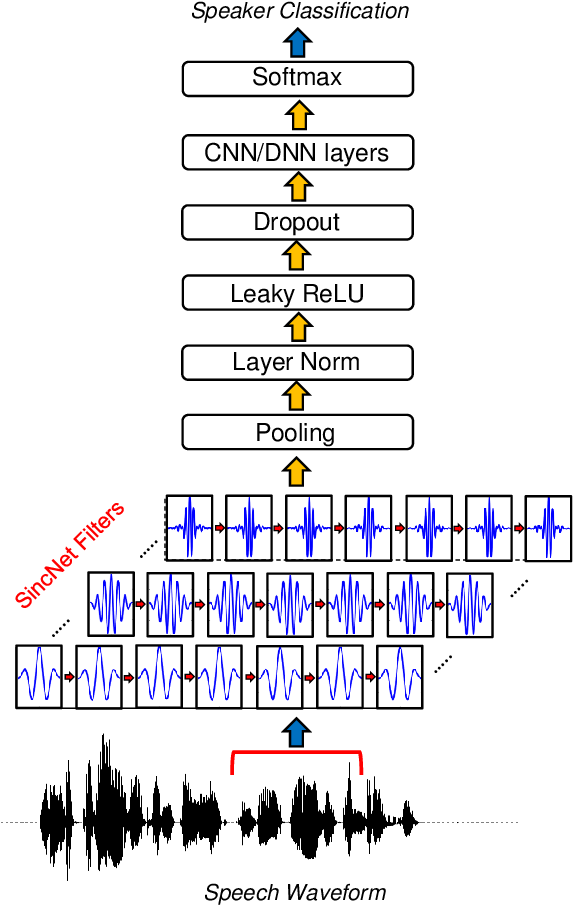
\includegraphics[width=120mm, keepaspectratio]{figures/sincnet-nn.png}
	\caption{SincNet architektúra~\cite{sincnet}.}
	\label{fig:sincnet-nn}
\end{figure}
\ \\
\newline
A SincNetet a TIMIT (462 beszélő) és Librispeech (2484 beszélő) adatbázisokkal tanították.
A beszédminták elejéről a szüneteket eltávolították, és LibriSpeech esetén azokat a mintákat, amelyek tartalmaztak legalább 125 ms hosszú szünetet, annak mentén feldarabolták. A TIMIT adatbázisnál egy beszélőtől 5 mintával tanítottak és 3 mintával teszteltek, míg LibriSpeechnél véletlenszerűen választott 12-16 másodperces mintákkal tanítottak és 2-6 másodpercesekkel teszteltek.
\newline
\begin{table}[!ht]
	\begin{tabular}{*3l} \toprule
		\bfseries Rendszer & \bfseries TIMIT & \bfseries LibriSpeech \\ \midrule
		DNN-MFCC & 0,99 & 2,02 \\
		\rowcolor{gray!10} 
		CNN-FBANK & 0,86 & 1,55 \\
		CNN-Raw  & 1,65 & 1,00 \\
		\rowcolor{gray!10} 
		SINCNET & 0,85 & 0,96 \\
		\bottomrule
		\hline
	\end{tabular}
	\centering
	\caption{Szöveg-független azonosítás eredményei adatbázisok szerint.}
	\label{fig:sincnet-identification}
\end{table}
\ \\
A \ref{fig:sincnet-identification}-es táblázat a CER (Classification Error Rate [\%]) hiba rátát mutatja. E szerint a SincNet jobban teljesít az MFCC, FBANK és nyers hullámformákkal tanított CNN-eknél mindkét adatbázis esetében, bár látható, hogy a sima CNN és a SincNet között minimális a különbség.
\newline
\begin{table}[!ht]
	\begin{tabular}{*3l} \toprule
		\bfseries Rendszer & \bfseries d-vector & \bfseries DNN-class \\ \midrule
		DNN-MFCC & 0,88 & 0,72 \\
		\rowcolor{gray!10} 
		CNN-FBANK & 0,60 & 0,37 \\
		CNN-Raw  & 0,58 & 0,36 \\
		\rowcolor{gray!10} 
		SINCNET & 0,51 & 0,32 \\
		\bottomrule
		\hline
	\end{tabular}
	\centering
	\caption{Szöveg-független ellenőrzés (verifikáció) eredményei.}
	\label{fig:sincnet-verification}
\end{table}
\ \\
\newline
A SincNettel nem jellemző vektorokat képeztek és a köztük lévő távolságot használták a hasonlóság mérésére, hanem osztályozással használják. Ebben az esetben zárt-halmazú beszélőazonosításról beszélünk. Ez sokkal kevésbé flexibilis, mert új beszélő esetén mindig újra kell tanítani a hálózatot, de cserébe jobb teljesítményre képes. A \ref{fig:sincnet-verification} ábrán egy d-vector nevű hangvektorokat képző neurális hálózatot hasonlítottak össze a SincNettel. Beszélőellenőrzés esetén a SincNet sokkal jobb EER-t ért el.
\newpage
\subsection{VoxCeleb2: Deep Speaker Recognition}

A VoxCeleb1 és VoxCeleb2 (2018) nagy méretű, beszélőfelismerés céljából készült adatbázisok. Az előbbi több mint 1000, utóbbi pedig több mint 6000 hangmintát tartalmaz hírességektől. Az adatbázisok felépítésének részleteit a \ref{voxceleb1} és \ref{voxceleb2} fejezetek ismertetik. Mindkét adatbázissal végeztek méréseket különböző neurális hálózatokkal, de a legjobb eredményeket illetve nyílt-halmazú beszélőfelismerést a VoxCeleb2-vel érték el~\cite{voxceleb2}.
\newline
\newline
Bemutatják a VGGVox nevű CNN alapú neurális hálózatot, amelyet spektrogramokkal tanítottak és hangvektorokat hoz létre. Előnye ennek a megoldásnak, hogy nyílt-halmazú beszélőfelismerésre használható, új beszélő esetén nem szükséges újra tanítani a hálózatot. 
\newline
\newline
Módosított VGG-M és ResNet architektúrákkal kísérleteztek. A modelleket contrastive loss veszteségfüggvénnyel tanították és előtanításra egy softmax réteget használtak keresztentrópiával, ami javította a modell teljesítményét. Tanító adathalmaznak a VoxCeleb2 adatbázist használták és a tesztelést a VoxCeleb1-el végezték. A méréseket EER és a \ref{eq:cdet} detektálási költség függvény szerint értékelték ki,

\begin{equation} \label{eq:cdet}
C_{det} = C_{miss} \cdot P_{miss} \cdot P_{target} + C_{fa} \cdot P_{fa} \cdot (1 - P_{target})
\end{equation}

ahol \emph{C\_miss} és \emph{C\_fa} alkalmazás specifikus paraméterek a hamis negatív és hamis pozitív hibák költsége, \emph{P\_miss} és \emph{P\_fa} pedig a hibák előfordulásának valószínűségét jelzik. \emph{P\_target} annak a valószínűsége, hogy a rendszer két olyan mintát hasonlít össze, amely egy embertől származik.
\newline
\begin{table}[!ht]
	\begin{tabular}{*4l} \toprule
		\bfseries Rendszer & \bfseries Tanítóhalmaz & \bfseries $C_{min}^{det}$ & \bfseries EER \\ \midrule
		I-vectors + PLDA & VoxCeleb1 & 0,73 & 8,8 \\
		VGG-M (Softmax) & VoxCeleb1 & 0,75 & 10,2 \\
		VGG-M & VoxCeleb1 & 0,71 & 7,8 \\
		VGG-M  & VoxCeleb2 & 0,609 & 5,94 \\
		ResNet-34 & VoxCeleb2 & 0,549 & 4,83 \\
		ResNet-50 & VoxCeleb2 & 0,429 & 3,95 \\
		\bottomrule
		\hline
	\end{tabular}
	\centering
	\caption{Beszélő ellenőrzés (verifikáció) eredményei.}
	\label{fig:sincnet-verification}
\end{table}

\newpage

\subsection{Utterance-level Aggregation for Speaker Recognition in the Wild}

A 2019-es cikk két fő témája egy olyan neurális hálózat létrehozása, amely képes különböző hosszúságú hangmintákból jellemző vektorokat képezni és olyan hangminták vizsgálata amelyek irreleváns zajokat is tartalmaznak~\cite{speaker_in_the_wild}.

\begin{figure}[!ht]
	\centering
	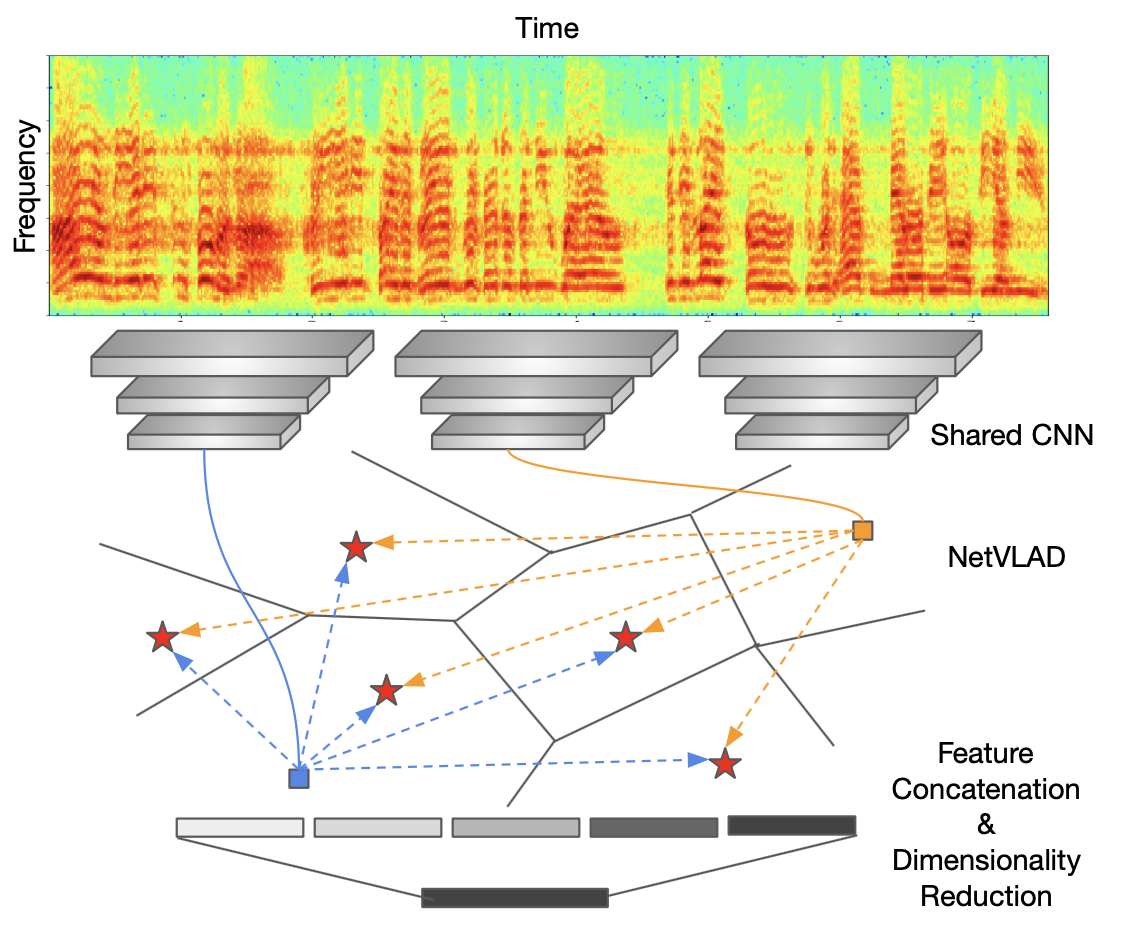
\includegraphics[width=150mm, keepaspectratio]{figures/frame-cnn.png}
	\caption{Neurális hálózat architektúra~\cite{speaker_in_the_wild}.}
	\label{fig:frame-cnn}
\end{figure}
\ \\
\newline
\newline
A hálózat három részből áll. Először egy módosított ResNet architektúrát használnak a keretszintű vektorok előállítására spektrogramokból. Az ábrán látható megosztott CNN-t hívjuk trönk hálózatnak. A keretszintű vektorok aggregálását a NetVLAD illetve GhostVLAD (Vector of Locally Aggregated Descriptors módszeren alapuló) hálózatokkal végzik. Legvégül egy FC (Fully Connected) réteget használnak a dimenzió 512-re csökkentésére.
\newline
\newline
A teljes modell end-to-end tanítására a VoxCeleb2 adatbázist használták és tesztelésként beszélőellenőrzést (verifikációt) mértek a VoxCeleb1-en.
\begin{figure}[!ht]
	\centering
	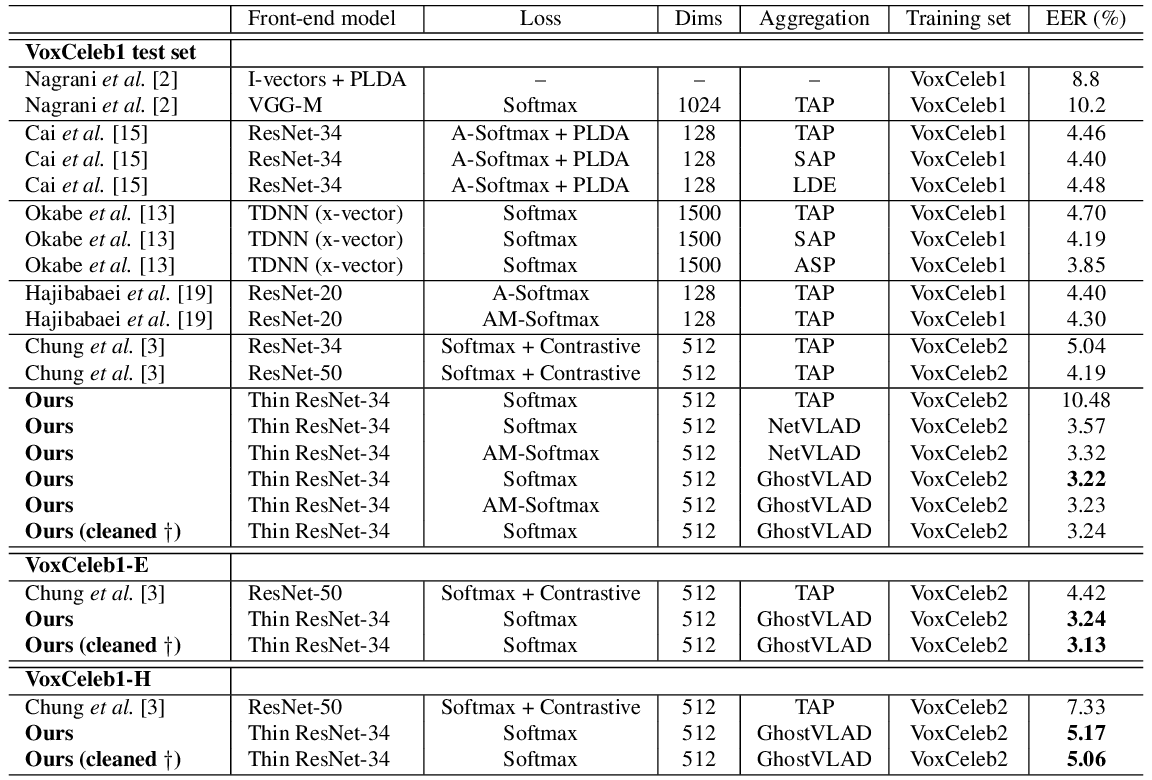
\includegraphics[width=150mm, keepaspectratio]{figures/frame-cnn-results.png}
	\caption{Neurális hálózat architektúra~\cite{speaker_in_the_wild}.}
	\label{fig:frame-cnn-results}
\end{figure}
\ \\
A \ref{fig:frame-cnn-results} táblázat mutatja a verifikációval mért EER-eket az akkori legkorszerűbb rendszerekkel szemben. Az addigiaknál lényegesen jobb EER-t értek el ezzel a módszerrel.

\section{A hangminták hossza}

Az eddigi rendszerekre hagyatkozva elmondható, hogy körülbelül 1-15 másodperces mintákkal tanították a neurális hálózatokat. Ez függ a beszédadatbázisban lévő hangminták méretétől, az előfeldolgozástól, és az határozza meg, hogy hiperparaméter optimizáció során mi bizonyul a legjobb értéknek. Ez rendszerenként változó. A \ref{section:modern_speaker_recognition} fejezetben ismertetett rendszerek és a voicemap kísérletek (\ref{section:voicemap_expermiments} fejezet) a következő eredményeket mutatták:

\begin{itemize}
	\item Deep speaker: 1-5 másodperces hangmintákból képzett 20-dimenziós MFCC-t használtak tanításhoz.
	\item LibriSpeech: 12-16 másodperces mintákkal tanítottak
	\item VoxCeleb2: 3 másodperces mintákból képzett spektrogrammokat használtak.
	\item Speaker Recognition in the Wild: Átlagosan 7-8 másodperces mintákat használnak (VoxCeleb2 adatbázis)
	\item voicemap: 3 másodperces minta volt a legjobb optimizálás után.
\end{itemize}

\section{Mérési környezet}

A mérésekhez a Google Colaboratoryt használtam, amely gépi tanulási kutatások és oktatás céljából felhő alapú környezetet biztosít. Hozzáférni Google fiókkal lehet, egy felhasználó egy virtuális gépet és egy Jupyter Notebookot kap. Választhatunk, hogy  a notebook a Python 2-es vagy 3-as verzióját támogassa, illetve, hogy CPU-n, GPU-n vagy TPU-n szeretnénk tanítani. A Tensor Processing Unit (TPU) a Google által fejlesztett gyorsító hardver egység Tensorflows tanításokhoz.
\newline
\newline
Az erőforrásokhoz fájlrendszert is kapunk. Ehhez hozzácsatolhatjuk a Google Drive fiókunkat, így elérhetjük a rajta tárolt adatokat. A notebookon keresztül elérjük a mögötte futó Linuxot is, lehet terminál parancsokat futtatni ha \emph{!} vagy \emph{\%} jelöléssel kezdjük a sort. Ez lehetővé teszi azt is, hogy pl. kisebb méretű dolgokat \emph{wget}tel töltsünk le vagy navigáljunk a fájlrendszerben, létrehozzunk új mappákat vagy töröljünk, áthelyezzünk fájlokat. Ugyan egyszerre több notebookot használhatunk, a fájlrendszer és a hardveres erőforrások ezek között megosztottak.

\subsection{Adatok előfeldolgozása}

Az előfeldolgozó szkript a TIMIT adatbázis esetében a hangmintákról eltávolítja a NIST Sphere fejlécet és a mondat előtti és utáni szüneteket. Ezután normalizálja a hangmintákat. A CMU Arctic esetében a hangminták alapból normalizálva vannak, ezért csak azonos méretűre kell vágni őket az egységes bemeneti dimenziók érdekében (ahogy a TIMIT esetében is).

\section{WaveNet classifier}

A \emph{WaveNet classifier} egy módosított WaveNet architektúra beszélőidentifikációhoz.

\subsection{WaveNet}

A WaveNet egy mély neurális hálózat audio hullámformák generálásához, amelyet a Google DeepMind publikált 2016-ban. Az ötletet az akkori felfedezések adták neurális autoregresszív generatív modellezés terén, amelyeket komplex eloszlások, például képek modellezésére használtak. Ezt felhasználva audio hullámformák generálásában új eredményeket értek el~\cite{wavenet}.

\begin{itemize}
	\item Képes olyan természetes hangzású beszéd hullámformák generálására, amit korábban parametrikus vagy konkatenatív beszédszintézissel sosem értek el. 
	\item Az audio hullámformák generáláshoz szükséges nagy receptív mezőt hatékonyan, nyújtott kauzális konvolúciókkal implementálja.
	\item Ha a modellt a beszélők identitásával tanítják, képes új hangok generálására.
	\item A zene generálás és a beszédfelismerés terén is ígéretesnek bizonyult.
\end{itemize}

\subsubsection{Nyújtott kauzális konvolúció}

A modell autoregresszív, vagyis a kimenete korábbi időpillanatokban felvett értékeitől függ. Ez azért fontos, mert a WaveNet egy generatív modell. A generált hullámforma \emph{t}-edik időpillanatbeli értéke nem függhet jövőbeli értékektől. A kauzalitás legegyszerűbb implementációja ha legalább \emph{kernel-1} méretű paddinget adunk a konvolúcióhoz.

\begin{figure}[!ht]
	\centering
	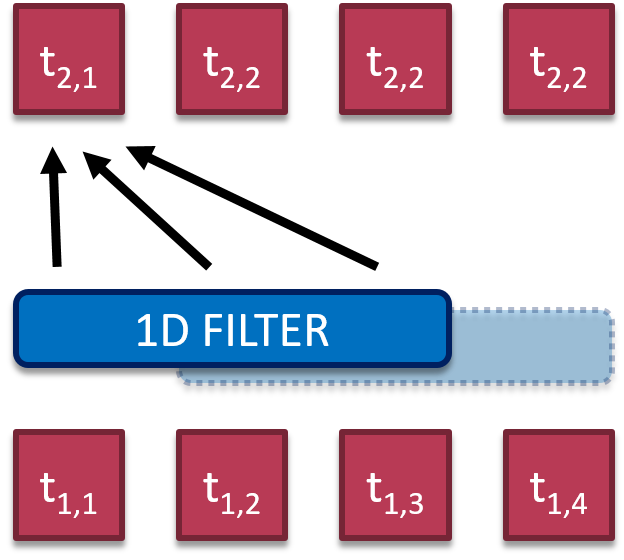
\includegraphics[width=80mm, keepaspectratio]{figures/1d-conv.png}
	\caption{1D nem kauzális konvolúció.}
	\label{fig:1d_noncausal_conv}
\end{figure}

\begin{figure}[!ht]
	\centering
	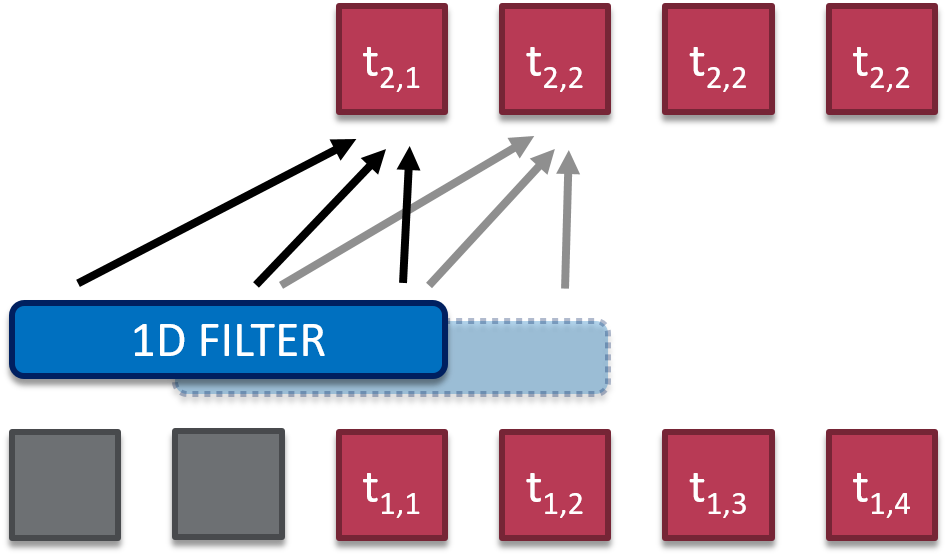
\includegraphics[width=120mm, keepaspectratio]{figures/1d-causal-conv.png}
	\caption{1D kauzális konvolúció paddinggel.}
	\label{fig:1d_causal_conv}
\end{figure}

\newpage

A \ref{fig:1d_noncausal_conv} ábra egy nem kauzális 1D konvolúciót mutat. A $t_{i, j}$ az i-edik rétegbeli j-edik neuron. Látható, hogy a $t_{2,1}$ jövőbeli időpillanatokból kap értékeket a szűrőn keresztül. Ennek megoldása a szűrő eltolása padding segítségével. Ezt szemlélteti a \ref{fig:1d_causal_conv} ábra, ahol az egyes neuronok csak korábbi időpillanatokból kapnak értékeket. 
\newline
\newline
A beszéd generálásánál a \emph{t}-edik időpillanatban a hullámforma értéke a korábbi adatoktól függ. Ahhoz, hogy magas frekvenciájú, pl. 16 kHz frekvencián mintavételezett 
hangadattal tanítsuk a hálózatot nagy receptív mezőre van szükség. A receptív mező az a szélesség, amit a szűrő lát a bemenetből. 16 kHz esetén egy másodpercnyi jelet 16000 szám reprezentál. Ahhoz, hogy a hálózat helyesen jósolja meg a következő generált értéket, a hosszú távú dependenciákat figyelembe kell vennie, tehát a receptív mező méretét elég nagyra kell megválasztani. A probléma ekkora mezők esetén, hogy sok konvolúciós réteget igényelnek (egy korábbi időpillanatbeli adat plusz egy konvolúciós réteget igényel), ami növeli a számítási komplexitást.
\newline
\newline
A nyújtott konvolúciók erre adnak hatékony megoldást. A filter meghatározott távolságokkal kihagy valamennyi inputot, majd figyelembe vesz egyet. Egymás utáni rétegekben a nyújtási tényezőt exponenciálisan növelve a receptív mező is exponenciálisan fog nőni.

\begin{figure}[!ht]
	\centering
	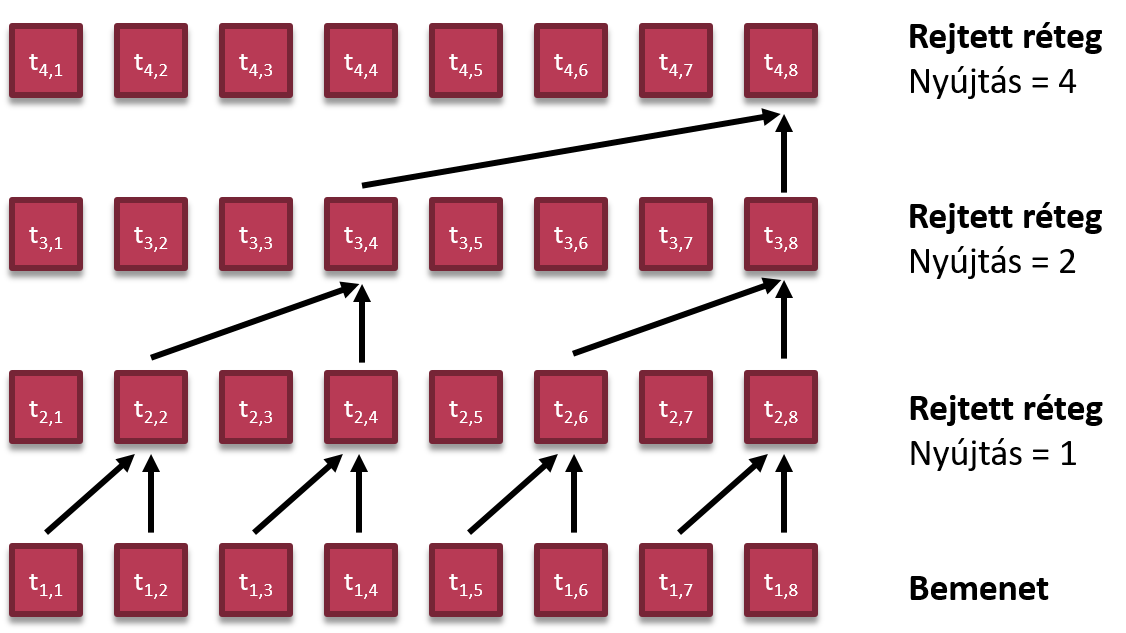
\includegraphics[width=150mm, keepaspectratio]{figures/1d-dilated-conv.png}
	\caption{1D nyújtott kauzális konvolúciós rétegek.}
	\label{fig:1d_dilated_conv}
\end{figure}

\subsubsection{SoftMax eloszlás}
A WaveNet SoftMax réteget használ a $p(x_t|x_1,\dots,x_t)$ feltételes valószínűségi eloszlás modellezésére.
Az audio jeleket általában 16 bites egészekkel kódolják, amelyek 65536 értéket vehetnek fel. Ebben az esetben a SoftMax rétegnek 65536 valószínűséget kell kimenetként adnia, melyek összege 1. A $\mu$-law kvantálást alkalmazva a beszédjel 256 biten kódolható és később az inverz transzformációval jó minőségben visszaállítható.
\newline
\newline
Az emberi hallás sokkal érzékenyebb alacsony amplitúdójú hangok kvantálási zajára, mint a magasabbakéra. Erre alapozva a $mu$-law kvantáló a jelet egy logaritmikus függvénnyel kvantálja úgy, hogy az alacsonyabb amplitúdójú jelek nagyobb felbontással (több bittel), a magasabbak pedig kisebbel lesznek kódolva. Ez növeli a SoftMax réteg hatékonyságát is, mert nagyobbak lesznek a valószínűségek közötti különbségek.
\newline
\newline
A tanítást a WaveNet klasszifikációs problémaként kezeli. A bemeneteket OneHot kódolással adjuk meg, a SoftMax réteg pedig az így kódolt egészekre ad valószínűségi eloszlást.

\subsubsection{Reziduális blokkok}

A WaveNet architektúra egymáshoz csatolt reziduális blokkokból és ún. kapcsolat-ugrásokból (skip-connection) épül föl. A reziduális hálózatok előnye, hogy orvosolják az elenyésző gradiens problémát, így sokkal mélyebb hálózat építhető.

\begin{figure}[!ht]
	\centering
	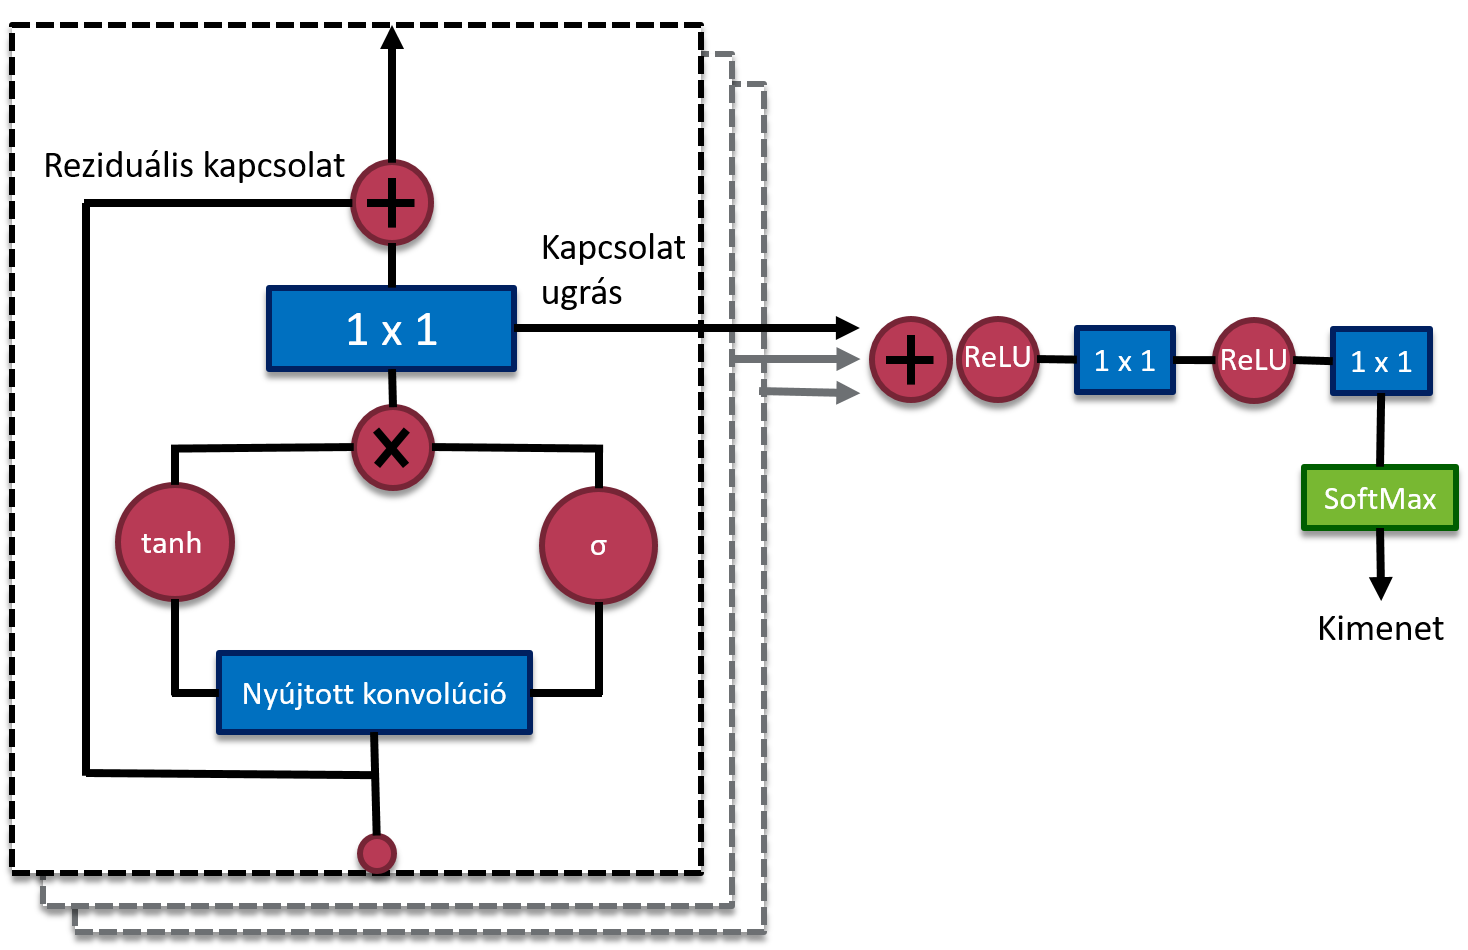
\includegraphics[width=150mm, keepaspectratio]{figures/wavenet_arch.png}
	\caption{WaveNet architektúra.}
	\label{fig:wavenet_arch}
\end{figure}

Egy reziduális blokk bemenete egy 2x1-es konvolúciós rétegen megy keresztül. Balra egy \emph{tanh}, jobbra egy szigmoid aktivációs függvényen haladnak át, majd elemenkénti szorzás és 1x1 konvolúció után egyrészt átugorja a reziduális kapcsolatot, illetve azzal együtt bemenetként szolgál a következő reziduális egységnek. Az 1x1 konvolúciós rétegek a dimenzionalitás változtatására szolgál. Külön 1x1 konvolúciós szűrők skálázzák a kimenetet a következő reziduális blokk bemenetére, és a kapcsolat-ugrásokhoz.

\subsection{Módosított WaveNet architektúra}

A módosított WaveNet architektúra segítségével a WaveNetet beszélőfelismerésre használhatjuk.
\bigskip
\begin{python}
	from WaveNetClassifier import WaveNetClassifier
	
	wnc = WaveNetClassifier((96000,), (10,), kernel_size = 2, dilation_depth = 9,
	                         n_filters = 40, task = 'classification')
	
	wnc.fit(X_train, y_train, validation_data = (X_val, y_val), epochs = 100,
	        batch_size = 32, optimizer='adam', save=True, save_dir='./')
	
	y_pred = wnc.predict(X_test)
	
\end{python}
\bigskip
A WaveNetClassifier objektum paraméterei:

\begin{itemize}
	\item \emph{input\_shape}: Bemeneti dimenziók tuple formájában. Például ha a bemenet egy 6 s hosszú hullámforma 16 kHz-en mintavételezve, a bemeneti dimenziók (96000,)
	\item \emph{output\_shape}: Kimeneti dimenziók tuple formájában. Például ha 100 osztály szerint klasszifikálunk, a kimeneti dimenziókból képzett tuple (100,).
	\item \emph{kernel\_size}: A konvolúciós filter/kernel mérete a reziduális blokkokban.
	\item \emph{dilation\_depth}: A reziduális blokkok száma.
	\item \emph{n\_filters}: A konvolúciós filterek száma a reziduális blokkokban.
	\item \emph{task}: Klasszifikáció vagy regresszió.
	\item \emph{regression\_range}: A regresszió céltartománya lista vagy tuple formátumban.
	\item \emph{load}: Előző WaveNetClassifier betöltése (bool).
	\item \emph{load\_dir}: A betölteni kívánt modell könyvtára.
\end{itemize}

\subsection{Eredmények}

A WaveNet classifiert TIMIT és CMU Arctic beszédadatbázisokkal teszteltem. A TIMIT beszédkorpusszal csak kevés beszélő esetén ért el jó eredményt, több mint 20 beszélő esetén a modell nem tanult. Ennek valószínűsített oka, hogy a TIMIT adatbázis beszélőnként 10 hangmintát tartalmaz.

\setlength\arrayrulewidth{0.6pt}

\begin{table}[!ht]
	\begin{tabular}{l|l} \toprule
		\bfseries Beszélők száma & 18 \\
		\rowcolor{gray!10}
		\bfseries Minta/beszélő & 100\\
		\bfseries Minta össz. & 1800 \\
		\rowcolor{gray!10}
		\bfseries Minta hossza & 4000 \\
		\bfseries Epochok száma & 43\\
		\rowcolor{gray!10}
		\bfseries Hiba & 0.0013 \\ 
		\bfseries Pontosság & 1.0 \\ 
		\bottomrule
		\hline
	\end{tabular}
	\centering
	\caption{Paraméterek CMU Arctic adatbázissal.}
	\label{fig:wavenet-arctic}
\end{table}
\ \\
A TIMIT TRAIN 630 beszélőt tartalmaz hangmintákat. Először lefuttattam rajta egy módosított előfeldolgozó szkriptet (LibriSpeech respository része), ami levágja a szüneteket a hangminták elejéről és végéről a WRD fájlnak megfelelően, majd normalizálja az amplitúdókat. ezekből kiválogattam azokat, amelyek legalább 2,5 mp hosszúak voltak, és beszélőnként 2:1 arányban tanító és teszthalmazra daraboltam őket.
Kevés, 10 beszélővel és 2,5 másodperces hangmintákkal tanítva, a teszt adathalmazon a hálózat 96.799 \%-os pontosságot ért el.
\newline
\newline
A CMU Arctic adatbázisokat letöltöttem a Google Colaboratory-s fájlrendszerre és egy mappa alá mozgattam őket. Ehhez csak az adatbázis kódjára volt szükség, mindegyik azonos kezdetű url-en található.
A CMU Arctic 16 bit-es wav fájlokat tartalmaz. Normalizálásként minden mintavételezett értéket leosztottam a maximális hosszal ($2^15 + 1$), hogy 0 és 1 közötti értéket vegyenek fel.
\newline
\newline
Tanítómintáknak 2-3 másodperces részeket választottam. A megfelelő hosszú wav fájlokból kivágtam a [0:40000] részt, így pontosan $40000/16000 = 2,5$ s-os szeleteket kaptam. Mind a 18 adatbázisból kiválasztottam 100 ilyen mintát. Ezeket véletlenszerűen összekevertem és ez az 1800 elemű halmazzal tanítottam. Az epochok száma 200 volt, de mivel a tanítás a 43-44. epochnál már 1-es pontosságot és közel 0 veszteséget mutatott, leállítottam a folyamatot. 
\newline
\newline
\begin{figure}[!ht]
	\centering
	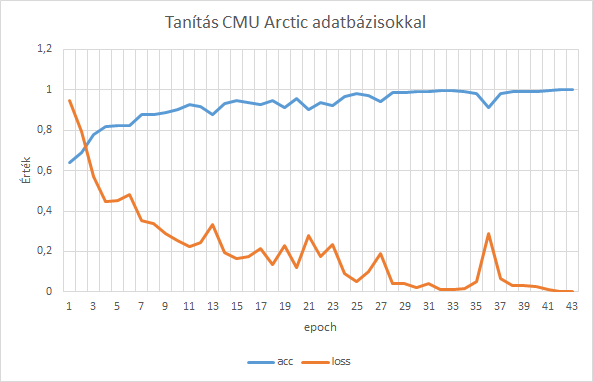
\includegraphics[width=150mm, keepaspectratio]{figures/wavenet-train-cmu-arctic.png}
	\caption{WaveNet tanítása CMU Arctic adatbázisokkal.}
	\label{fig:wavenet-train-cmu-arctic}
\end{figure}
A teszthalmazba a tanítómintákon kívüli minimum 40000 hosszú wav fájlok kerültek, összesen 10152 minta.
Az elvárt kimeneteket one-hot kódoltam és kiértékeltem a modellt a tesztadatokon. A felismerés pontossága $97,3$ \% volt 18 ember esetén.

\section{Voicemap}

A \emph{voicemap} egy nyílt forráskódú deep learning projekt beszélőfelismerő feladatok elvégzéséhez. A GitHub repository tartalmazza a modell kódját, a tanítást, különböző kísérleteket és egy hiperparaméter-optimizált, előre tanított modellt. Az implementációhoz \emph{Kerast} illetve újabb verziókban \emph{Pytorchot} használ~\cite{voicemap_github}.
\newline
\newline
A projekt célja, hogy későbbiekben egy olyan általános, pip által telepíthető csomag legyen, ami könnyen felhasználható beszélőfelismeréssel kapcsolatos feladatok elvégzésére.

\subsection{A projekt általános felépítése}

Mivel a saját alkalmazásomban felhasználtam és átalakítottam a projekt egyes részeit,
röviden bemutatom a felépítését.

\begin{itemize}
	\item \emph{models.py}: A konvolúciós enkóder létrehozását és a sziámi hálózat építését végzi el.
	\item \emph{librispeech.py}: Keras szekvencia osztály Librispeech beszédadatbázisból származó hangminták tárolására, előfeldolgozására és generálására tanításhoz. Fő paraméterei a következők:
	\begin{itemize}
		\item \emph{subsets}: Mely LibriSpeech adathalmazokat tartalmazza.
		\item \emph{seconds}: Az ennél rövidebb időtartamú hangmintákat figyelmen kívül hagyja.
		\item \emph{stochastic}: Sztochasztikus módban a mintákból véletlenszerűen vágjuk ki a \emph{seconds} hosszúságú darabot.
		\item \emph{pad}: Padding esetén a rövidebb hangmintákat nullával feltöltve a megadott méretre alakíthatjuk. Sztochasztikus mód esetén véletlenszerűen oszlik el a hangminta előtti és utáni nullák száma.
	\end{itemize}
	
	A két legfontosabb függvénye:
	
	\begin{itemize}
		\item \emph{build\_verification\_batch}: A sziámi hálózat teszteléséhez generál olyan batchet, amelyben az ugyanattól és az eltérő beszélőktől származó hangmintapárok száma azonos (50\%-50\%). A batch egy eleme két hangmintából és egy címkéből áll, ami jelzi, hogy egyazon vagy más-más beszélőktől származnak.
		\item \emph{build\_n\_shot\_task(k, n)}: Visszaad egy segédhalmazt $n$ mintával minden egyes $k$ beszélőhöz és visszaad egy mintát, amiről a modellnek el kell döntenie, hogy melyik beszélőhöz tartozik.
	\end{itemize}
	\item \emph{utils.py}: Fő feladata az adatok preprocesszálása és az \emph{n\_shot\_task\_evaluation} függvény által az \emph{n-shot k-way} feladat kiértékelése. A few-shot kiértékeléshez alábbi argumentumokat adhatjuk meg:
	
	\begin{itemize}
		\item  \emph{model}: A tesztelendő modell.
		\item  \emph{dataset}: A tesztmintákat tartalmazó adathalmaz objektum.
		\item  \emph{preprocessor}: Előfeldolgozó függvény a minták csökkentett mintavételezésére és standardizálására.
		\item  \emph{num\_task}: A feladatok száma.
		\item  \emph{n}: Hány hangminta tartozik egy beszélőhöz a segédhalmazban.
		\item  \emph{k}: Ennyi beszélő, azaz osztály van a segédhalmazban.
		\item  \emph{network\_type}: Sziámi vagy klasszifikációs.
		\item  \emph{distance\_metric}: Sziámi hálózat esetén a hangvektorok közötti távolságmetrika.
	\end{itemize}
\end{itemize}

\subsection{Az implementált modellek}

A projekt két modellt vizsgál; egy sziámi neurális hálózatot (a konvolúciós sziámi hálózat részletes leírása a \ref{section:siamese_conv} fejezetben található) és egy sima konvolúciósat klasszifikációval. Mindkét hálózat alapja alapja egy konvolúciós enkóder, amely a nyers hangmintákból kinyeri a jellemzőket és hangvektorokat állít elő belőlük. Az enkóder hálózat a több egymást követő konvolúciós blokk áll. Egy konvolúciós blokk felépítése a \ref{fig:conv_encoder_block} ábrán látható. Ezek egy konvolúciós rétegből és regularizációs
rétegekből tevődnek össze.

\begin{figure}[!ht]
	\centering
	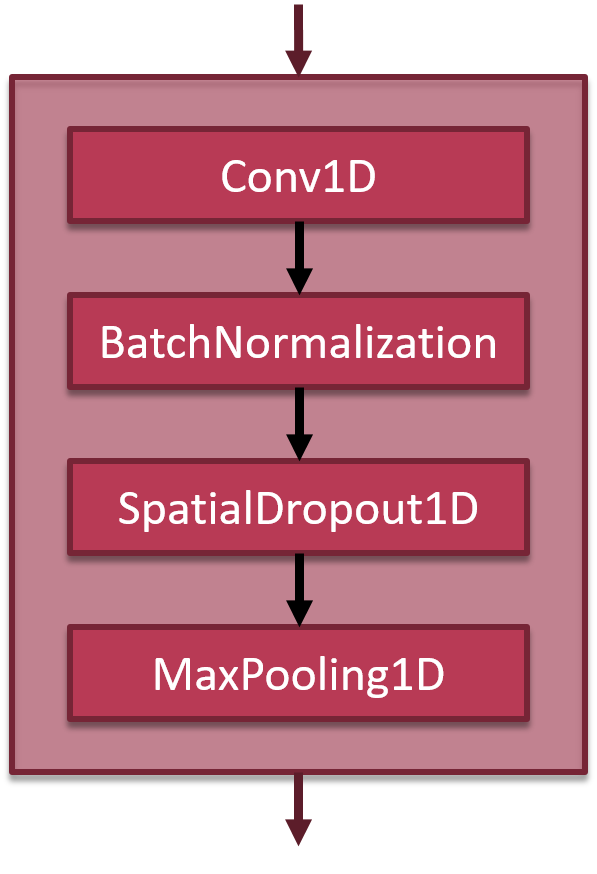
\includegraphics[width=80mm, keepaspectratio]{figures/conv_encoder_block.png}
	\caption{Egy konvolúciós enkóder blokk felépítése.}
	\label{fig:conv_encoder_block}
\end{figure}

\begin{itemize}
	\item Conv1D: 32-es méretű filterekkel, ahol a filterek száma arányosan nő azzal, hogy a blokk hányadik a sorban. Az aktivációs függvény \emph{ReLu}.
	\item BatchNormalization: Batchenként normalizálja az előző réteg kimeneteit úgy, hogy az átlag 0-hoz, a szórás 1-hez közelítsen. Regularizációra használják.
	\item SpatialDropout1D: Sima dropout réteg esetén az egyes neuronokat valamekkora valószínűséggel figyelmen kívül hagyjuk. Például egy [[1, 2, 3], [2, 3, 1]] tömbnek a kimenete sima dropout esetén lehet [[1, 0, 3], [0, 3, 1]], itt teljesen függetlenek egymástól a kinullázások. Spatial dropout esetén az adott dimenzió mentén mindent kinullázunk. Például [[1, 0, 3], [2, 0, 1]]. Regularizációra használják.
\end{itemize}
\ \\
Négy ilyen konvolúciós blokk követi egymást, majd további regularizáció: egy \emph{GlobalMaxPool1D} és egy \emph{Dense} réteg a hangvektor méretével.

\begin{figure}[!ht]
	\centering
	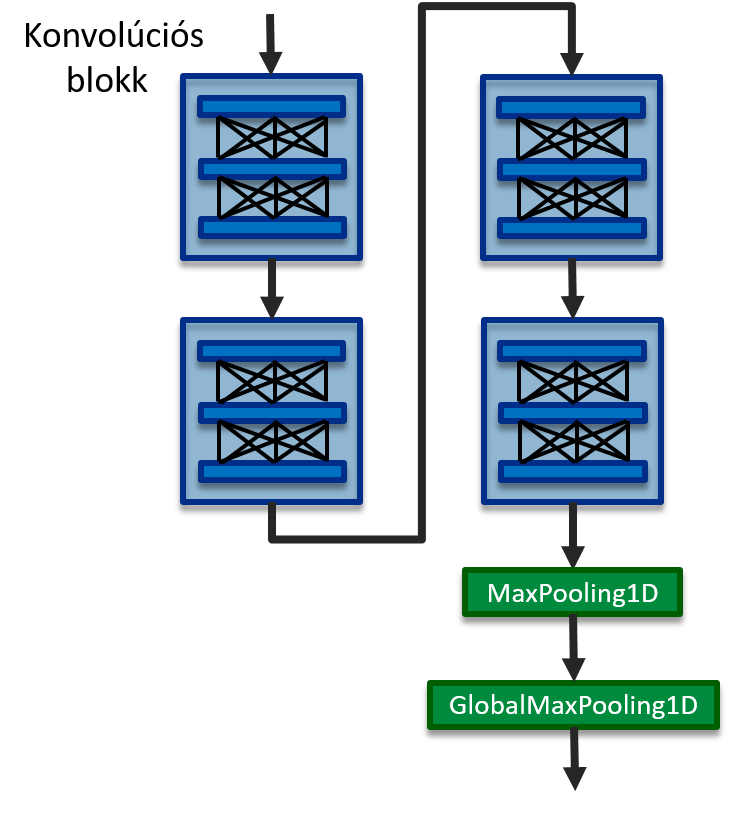
\includegraphics[width=100mm, keepaspectratio]{figures/conv_encoder.png}
	\caption{A konvolóciós enkóder felépítése.}
	\label{fig:conv_encoder}
\end{figure}
\ \\
A sziámi hálózat alapja két enkóder hálózat, amelynek súlyai megosztottak, tehát úgy is tekinthetünk rá, hogy egy enkóder hálózatra két bemenetet adhatunk. A hangminták a hálózaton áthaladva jellemző vektorokká alakulnak. Ezt a részt a konvolúciós enkóder végzi. Ezután a két vektor közötti távolságmetrikát a sziámi hálózat kiszámolja. Ezen távolság alapján számolja ki a veszteséget és javítja a súlyokat.
\ \\
Az implementált távolságmetrikák a következők:

\begin{itemize}
	\item \emph{weighted\_l1}: Az eredeti one-shot cikk szerinti távolságmetrika. $v_1$ és $v_2$ vektorokra $\sqrt{v_1-v_2}$.
	\item \emph{uniform\_euclidean}: Euklideszi távolság két vektor között.
	\item \emph{cosine\_distance}: Koszinusz távolság, azaz a két vektor által bezárt szög koszinuszát méri.
\end{itemize}

A kiszámolt távolság ezután minden esetben áthalad egy szigmoid aktivációs függvényű \emph{Dense} rétegen, ami $0$ és $1$ közé nyomja az eredményt.

\subsection{Beszédadatbázisok és generátorok}

A voicemap tanításhoz és teszteléshez a \emph{LibriSpeech} adatbázis \emph{dev-clean}, \emph{train-clean-100} és \emph{train-clean-360} adathalmazokat használja, amelyek sorban $40$, $251$ és $921$ különböző beszélőtől tartalmaznak nyers hangfájlokat.
\newline
\newline
Egy adathalmazt egy adatgenerátor osztály reprezentál ami a keras.util.Sequence osztályból származik. Az adatgenerátorok nagy adathalmazok esetén hasznosak, amikor az egész adathalmaz nem fér bele a memóriába. Ilyen esetekben egyesével generálnak adatokat.
\newline
\newline
A \emph{keras.util.Sequence} osztályból való leszármaztatás miatt az adatgenerátorban implementálni kell a \emph{\_\_len\_\_} és \emph{\_\_get\_item\_\_} függvényeket. Előbbi az adathalmaz méretét adja vissza, utóbbi annak indexelését teszi lehetővé. Továbbá biztosítja, hogy egy epochon belül egy mintával csak egyszer tanítjuk a modellt.

\subsection{Tanítás}

A sziámi és a sima klasszifikációs hálózat nagyrészt közös paraméterekkel rendelkeznek. A fő különbség, hogy míg a sziámi veszteségfüggvénye bináris keresztentrópia, és a veszteség az alapján dől el, hogy a hangminta pár egyazon vagy más beszélőktől származik, a klasszifikációs hálózat kategórikus keresztentrópiát használ, tehát a hangmintát megpróbálja besorolni $k$ osztály valamelyikébe $k$ beszélő esetén. A közös paraméterek:

\begin{itemize}
	\item hangminta hossza: 3 sec
	\item batchsize: 64
	\item filterek száma: 128
	\item jellemző vektor dimenzió: 64
	\item dropout: 0
	\item steps\_per\_epoch: 500
	\item kiértékelési feladatok száma: 500
	\item n\_shot\_klasszifikáció: 1
	\item k\_way\_klasszifikáció: 5
\end{itemize}

Tehát mindkét modell optimizált hiperparamétereket használ, \emph{Adam} optimizálót és veszteségfüggvényként keresztentrópiát. Egy epoch $500$ batch iterációból áll és egy batch méret $64$.
Az epochok végén három callback fut le.
\newline
\newline
Minden epoch végén kiértékelés történik: 500 \emph{1-shot 5-way} feladat átlagos eredménye jelzi a pontosságot. Amennyiben ez növekszik a modellről \emph{checkpoint} készül (\emph{ModelCheckpoint}).
Továbbá ha a kiértékelés során a pontosság nem nő, a \emph{ReduceLROnPlateau} csökkenti a tanulási rátát.


\subsection{Kísérletek és optimalizálás} \label{section:voicemap_expermiments}

A repositoryban számos kísérlet található a legjobb teljesítmény elérésére. A \emph{wide\_vs\_tall} szkript leméri, hogy a modell hogyan teljesít különböző hosszúságú hangmintákkal tanítva. A mérés alatt \emph{1-shot 5-way} feladatokkal, azaz 5 különböző beszélőtől 1-1 beszédmintával validálta a modellt~\cite{voicemap_medium}.

\begin{figure}[!ht]
	\centering
	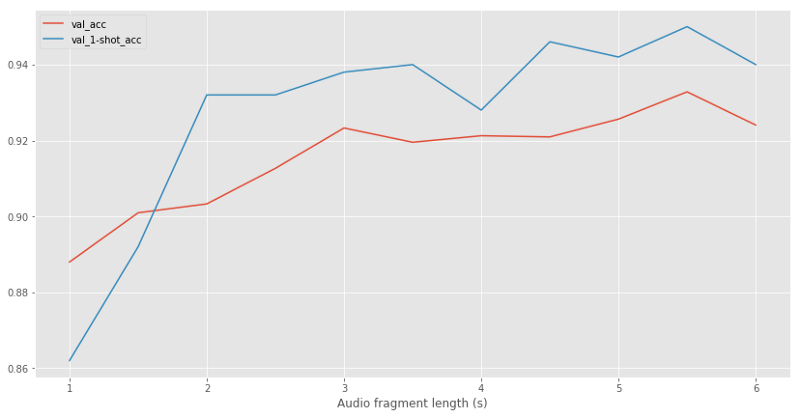
\includegraphics[width=150mm, keepaspectratio]{figures/voicemap-wide-vs-tall.png}
	\caption{Voicemap: Regisztrációs fázis.}
	\label{fig:voicemap-wide-vs-tall}
\end{figure}

A \ref{fig:voicemap-wide-vs-tall} ábrán látható, hogy a hangminta méretét növelve a modell valóban jobban tanul, de a több adat miatt megnövekedik a tanítási idő és több memóriára van szükség. A grafikon mutatja, hogy 3 másodperc után a validáció stagnálni kezd, ezért az erőforrásokat és a tanítási időt figyelembe véve ez tűnik a legjobb választásnak.
\newline
\newline
A \emph{grid\_search\_siamese\_network} szkript hiperparaméter optimizációt végez a sziámi hálózaton a filterek számát, a hangmintákból képzett vektorok hosszát és a dropoutot vizsgálva. A talált legjobb paraméterek:

\begin{itemize}
	\item filterek száma: 128
	\item jellemző vektor dimenzió: 64
	\item dropout: nincs
\end{itemize}
\ \\
A \emph{k\_way\_accuracy} kísérlet a hiperparaméter optimalizált modell teljesítményét méri le különböző \emph{n-shot k-way} feladatokkal. A pontosságot a \ref{fig:voicemap-n-shot-k-way} ábra mutatja.

\begin{figure}[!ht]
	\centering
	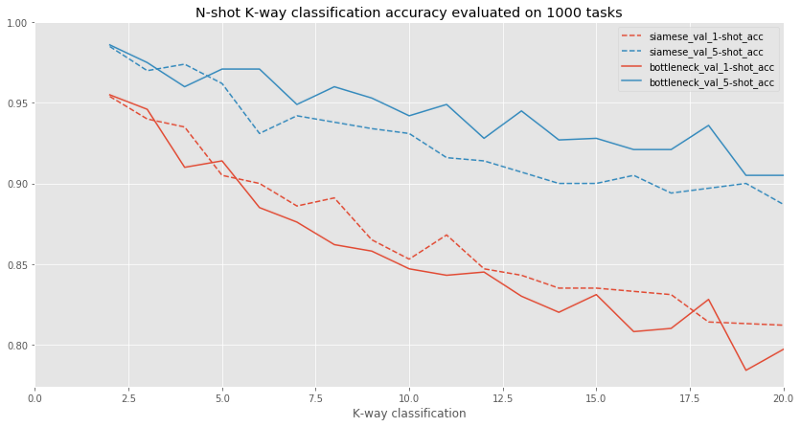
\includegraphics[width=150mm, keepaspectratio]{figures/voicemap-n-shot-k-way.png}
	\caption{Voicemap: n-shot k-way pontosság.}
	\label{fig:voicemap-n-shot-k-way}
\end{figure}
\ \\
\emph{1-shot k-way} feladatok esetén a sziámi hálózat átlagosan jobban teljesít sima klasszifikációsnál, de \emph{5-shot k-way} feladatok esetén már az utóbbi kerül fölénybe. Ez valószínűleg annak köszönhető, hogy 5 hangminta - beszélő párból a sima osztályozó hálózat már jobban meg tudta tanulni a beszélőket a sziáminál.


\begin{figure}[!ht]
	\centering
	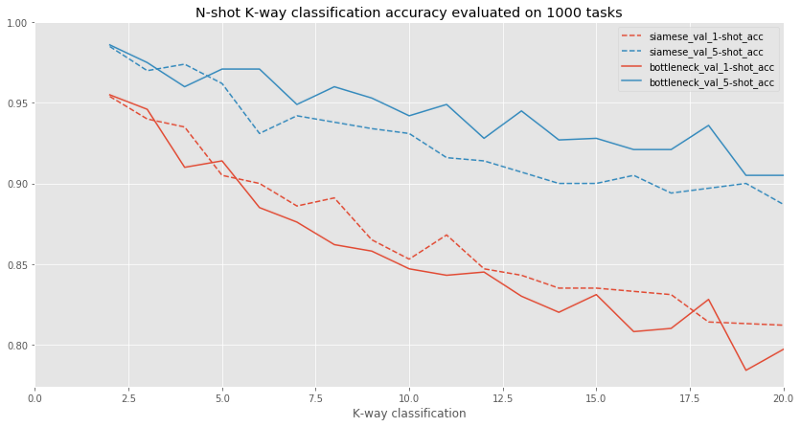
\includegraphics[width=150mm, keepaspectratio]{figures/voicemap-n-shot-k-way.png}
	\caption{Voicemap: n-shot k-way pontosság.}
	\label{fig:voicemap-n-shot-k-way}
\end{figure}

\newpage
\ \\
Lemértem sziámi hálózat esetén a contrastive loss és bináris keresztentrópia veszteségfüggvények közötti különbséget. Mindkét modellt az optimizált hiperparaméterekkel 50 epochon keresztül tanítottam.

\begin{figure}[!ht]
	\centering
	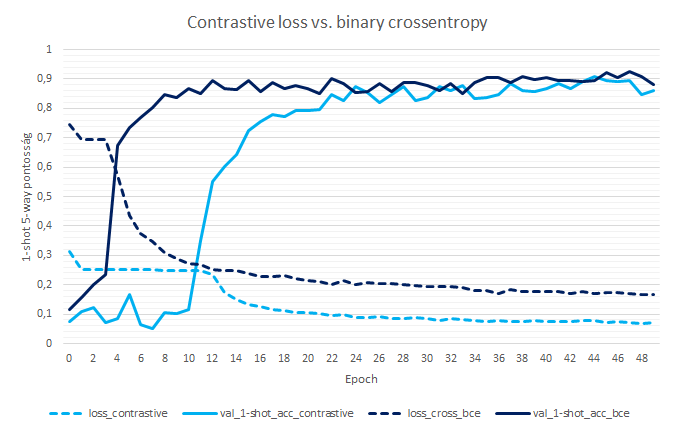
\includegraphics[width=150mm, keepaspectratio]{figures/contrastive_vs_bce.png}
	\caption{Voicemap: n-shot k-way pontosság.}
	\label{fig:contrastive_vs_bce}
\end{figure}
\ \\
A \ref{fig:contrastive_vs_bce} grafikon mutatja, hogy a \emph{1-shot 5-way} pontosság a 20. epochnál kezd 90\% fele konvergálni. A maximális pontosság contrastive lossnál a 44. epochnál 90,8\%, míg bináris keresztentrópia esetén a 47. epochnál 92,6\%.

\newpage

\subsection{Saját kísérlet: Triplet loss}


A sziámi hálózatoknak egy ismert költségfüggvénye a \emph{triplet loss} függvény. Ezt a \emph{gradient descent} módszerrel optimizálva tanítjuk a hálózatot. A triplet loss három bemenetet igényel, amelyek jelen példában a hangokból képzett jellemző vektorok. Az egyik egy rögzített hang vektora, ez az ún. \emph{anchor}. A másik kettő pedig egy pozitív és egy negatív minta. A pozitív ugyanattól a beszéltőtől származik mint az \emph{anchor} vektor, a másik különbözőtől~\cite{triplet_semi_hard}.
\begin{equation}\label{eq:4}
\mathcal{L}_{triplet}(A, P, N) = \max(d(A, P) - d(A, N) + m, 0)
\end{equation}
\ \\
A $d$ a távolságfüggvény, ami lehet például euklideszi távolság. A \emph{triplet loss} veszi az anchor és a pozitív meg az anchor és a negatív minta távolságainak különbségét, majd ezt eltolja az $m$ küszöbértékkel. Ha az előbbi pozitív ezt veszi eredményül, egyébként nullát.

\begin{figure}[!ht]
	\centering
	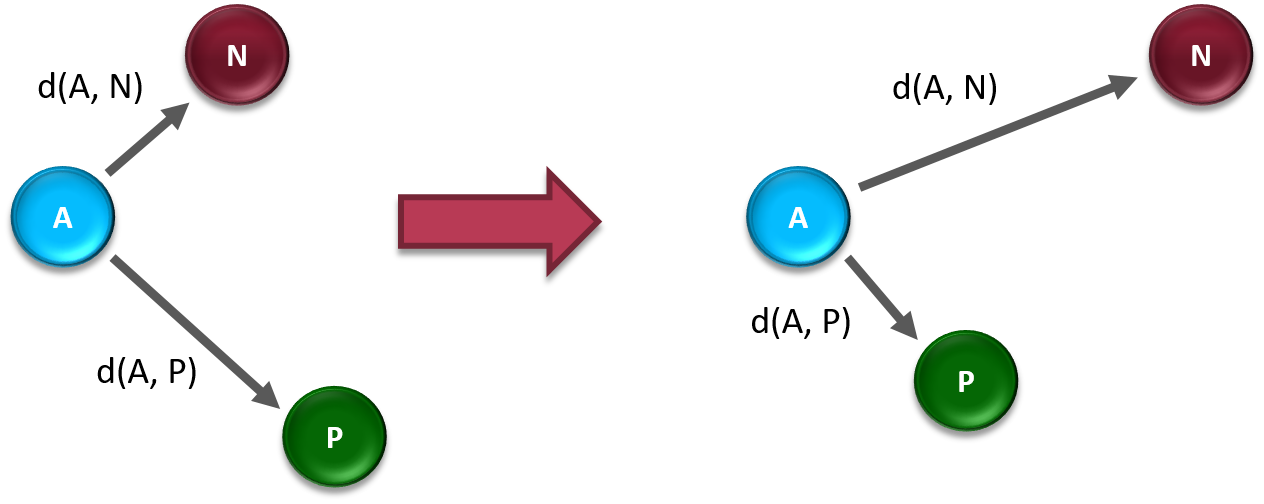
\includegraphics[width=100mm, keepaspectratio]{figures/triplet-loss.png}
	\caption{A triplet loss függvény csökkenti a távolságot a hasonló és növeli a különböző minták között.}
	\label{fig:triplet-loss}
\end{figure}
\ \\
Akkor jó a vektorok elhelyezkedése a metrikus térben, ha a hasonlók között a távolság kicsi, a különbözők között pedig nagy. Azt szeretnénk elérni, hogy
$d(A, P) \le d(A, N)$ fenn álljon. Átrendezve a $d(A, P) - d(A, N) \le 0$ egyenletet kapjuk. Ezt kielégíti a $d(A, P) = 0$, $d(A, N) = 0$ megoldás. A másik triviális megoldás, ha a pozitív és negatív minta kódolása ugyanaz lenne, ekkor ugyanis $d(A, P) = d(A, N)$ így $d(A, P) - d(A, N) = 0$. Szeretnénk, ha a neurális hálózat nem nullvektorokkal vagy azonos vektorokkal kódolná az összes képet, ezért hozzáadunk egy $m$ küszöbértéket az egyenlethez.

\begin{equation}\label{eq:5}
\begin{aligned}
d(A, P) + m \le d(A, N) \\
d(A, P) - d(A, N) + m \le 0
\end{aligned}
\end{equation}
\ \\
Ideális esetben a $d(A, P) - d(A, N) + m$ negatív, ilyenkor a veszteség 0. Ha nem így van, a triplet loss ezt a veszteséget adja vissza. A költségfüggvény a tanítóhalmazban lévő tripletekre alkalmazott triplet lossok összege. Ezt minimalizálva a \ref{fig:triplet-loss} ábrán látható távolságok csökkentése, növelése történik.
\newline
\newline
A tripletek kiválasztására többféle módszer létezik. A legegyszerűbb megoldás
-- amit én is használtam -- a véletlenszerű kiválasztás. Emelett a tripleteket három kategóriába sorolhatjuk~\cite{triplet_semi_hard}\cite{triplet_github}. Ezt a \ref{fig:triplet-type} ábra szemlélteti:
\begin{itemize}
	\item Könnyű (negatív) triplet: A 0 veszteségű tripletek, mivel $d(A, P) + m \le d(A, N)$.
	\item Nehéz (negatív) tripletek: A negatív közelebb van az anchorhoz mint a poztiív: $d(A, N) \le d(A, P)$
	\item Félnehéz (negatív) tripletek: Olyan tripletek, ahol a negatív nincs közelebb az anchorhoz mint a pozitív, de mégis nagyobb a veszteség nullánál: $d(A, P) \le d(A, N) \le d(A, P) + m$.
\end{itemize}

\begin{figure}[!ht]
	\centering
	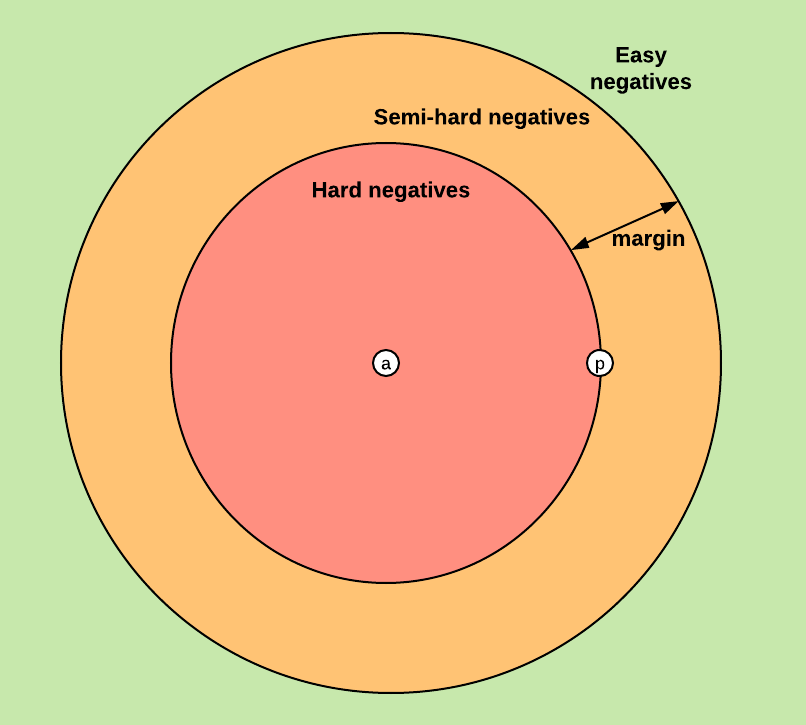
\includegraphics[width=120mm, keepaspectratio]{figures/triplet_type.png}
	\caption{A tripletek három típusa.}
	\label{fig:triplet-type}
\end{figure}

\ \\
Nehéz tripletek bányászása egy külön feladat és léteznek módszerek ún. offline (tanítás előtti) és online (tanítás közbeni) generálásra. Előnye, hogy gyorsabban konvergál a hálózat a veszteség minimuma felé. Ugyanakkor a FaceNet megjegyzi, hogy nehéz tripletekkel való tanítás az elején rossz lokális minimumhoz vezethet, ezért a félnehéz tripleteket ajánlja.

\subsubsection{Voicemap implementáció}

Létrehoztam egy bemenetként tripleteket fogadó neurális hálózatot \emph{triplet loss} veszteségfüggvénnyel (a triplet loss veszteségfüggvény részletes leírása a \ref{section:siamese_conv} fejezetben található). Egy bemenet egy olyan hangminta hármas (triplet), ami két azonos és egy különbözőtől beszélőtől tartalmaz hangmintát. 
\newline
\newline
A két azonos minta közül az egyik lesz az \emph{anchor} érték. Ehhez mérten számoljuk ki a pozitív (azonos beszélőtől származó) és negatív (különböző beszélőtől származó) távolságokat. 
\newline
\newline
Az alapja a konvolúciós enkóder. Ehhez csatlakozik három bemenet, a kimenetére pedig két lambda réteg ami a pozitív és negatív távolságokat számolja ki, majd még két lambda réteg kiszámolja a vektorok hosszát. A szubtrakciós réteg ezután a két kiszámolt vektort kivonja egymásból, ahogy a \ref{fig:triplet-network} ábrán látható.

\begin{figure}[!ht]
	\centering
	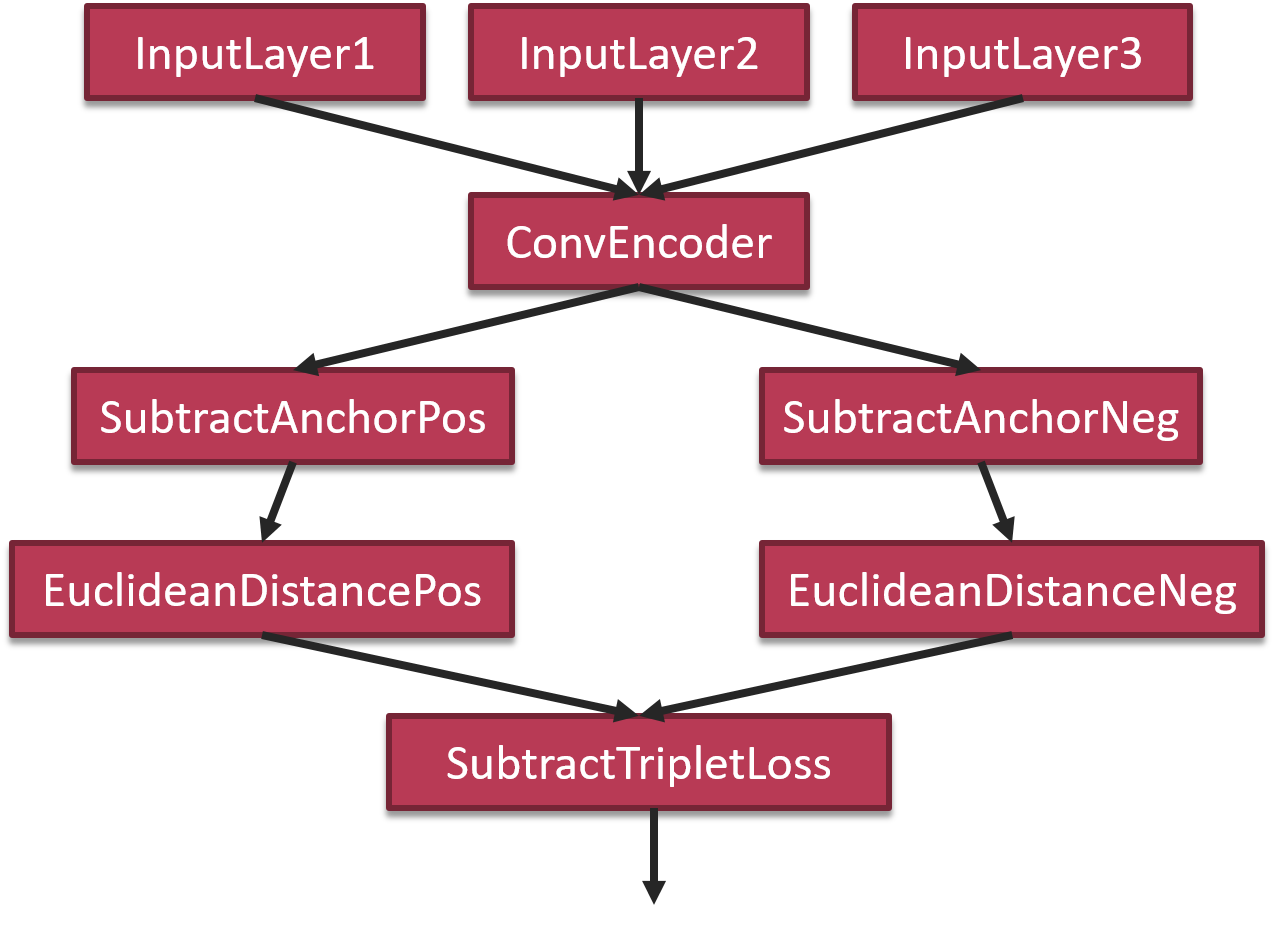
\includegraphics[width=120mm, keepaspectratio]{figures/triplet-network.png}
	\caption{Triplet hálózat.}
	\label{fig:triplet-network}
\end{figure}
\ \\
Tanításhoz a LibriSpeech adatbázist használtam. Ehhez módosítottam a \emph{LibriSpeechDataset} osztályt úgy, hogy képes legyen tripletekből álló batchek generálására is.
\newline
\newline
Az \emph{utils.py}-ben implementáltam magát a \emph{triplet loss} veszteségfüggvényt, módosítottam a BatchPreProcessor wrapper osztályt, hogy egységesen kezelje a triplet alakú tanítóadatokat a sziámi és sima konvolúciós bemenetekkel együtt, majd kiegészítettem az \emph{n\_shot\_task\_evaluation} függvényt úgy, hogy képes legyen \emph{k-way n-shot} feladat kiértékelést tripleteken is elvégezni.

\begin{figure}[!ht]
	\centering
	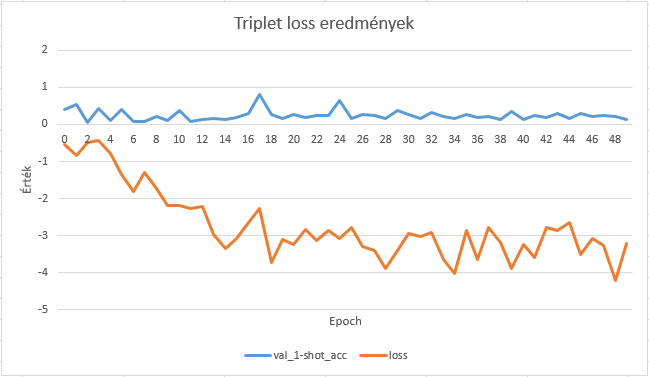
\includegraphics[width=150mm, keepaspectratio]{figures/triplet-loss-chart.png}
	\caption{Triplet lossal tanítás eredményei.}
	\label{fig:triplet-loss-chart}
\end{figure}
\ \\
A tanítás során minden batch végén 1-shot 5-way kiértékelés történik, azaz 5 beszélőtől egyelemű segédhalmazokkal próbálja a hálózat megtippelni, hogy melyik beszélőhöz tartozik a kérdéses hangminta.
\newline
\newline
A \ref{fig:triplet-loss-chart} grafikon azt mutatja, hogy az egyes epochok szerint hogyan változik a veszteség és a 1-shot 5-way pontosság. Látható, hogy a veszteség stagnálva, de csökken, ennek ellenére a validációs pontosság folyamatosan 0 és 1 között változik. A 17. és 24 epochnál megközelíti az 1-et, majd tovább romlik. A pontosság és a veszteség nem lassan, hanem egyáltalán nem konvergál, ezért feltételezhető, hogy nem a véletlenszerű tripletek kiválasztása a probléma. A tanítás nem volt sikeres.